\title{Machine Learning Practical - Assignment 1}
\author{s1247438}
\documentclass[12pt]{article}
\usepackage{caption}
\usepackage{subcaption}
\usepackage[pdftex]{graphicx} 
\usepackage[margin=1in]{geometry}    


\begin{document}

\maketitle


\subsection*{Introduction}
This coursework is focused on training a multi-layered neural network for digit classification on the MINST dataset. The aim of this coursework is to investigate the effect of learning rates, learning rate schedules and adaptive learning rates on the model training and final performance.

\subsection*{Methodology}
The neural network built for the purposes of this assignment is based on the Lab session code provided. After implementing schedules and learning rules the effect of their hyperparameters was investigated. This has been done by creating a parallelisable code allowing to run multiple neural network trainings simultaneously, making the most of computers with a large number of CPUs(~50). By running a higher number of experiments the effect of hyperparameters could be observed and the best ones could be chosen for each schedule. The performance of the models trained with these optimal hyperparameters were then compared.



\section*{Task 1 - Learning rate schedules}

The focus of the first section is to create and compare two different learning rate schedules : constant and exponential. The constant learning rate schedule uses a static learning rate that does not change during the training process and will then be taken as a baseline. The exponential learning rate is time-depended, the value changes as the time progresses. 
\[ n(t) = n_0*e^{(-t/r)}\] 
The equation contains two parameters n and r which dictate how quickly the learning rate decays. The aim being to start with higher learning rate and progressively decrease over time to make smaller adjustments. This section investigates different hyperparameter variations for both learning rate schedules.


\begin{figure}[h]
\centering
\begin{subfigure}{.5\textwidth}
  \centering
  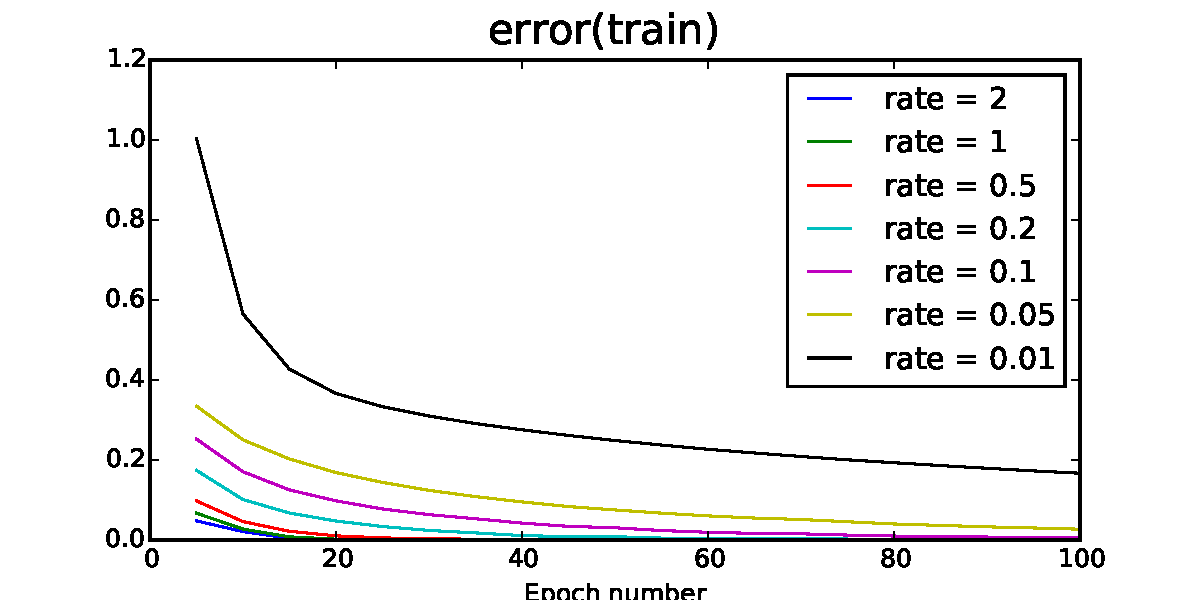
\includegraphics[width=7cm]{Task1/figures/Const_rule_error(train).pdf}
\end{subfigure}%
\begin{subfigure}{.5\textwidth}
  \centering
  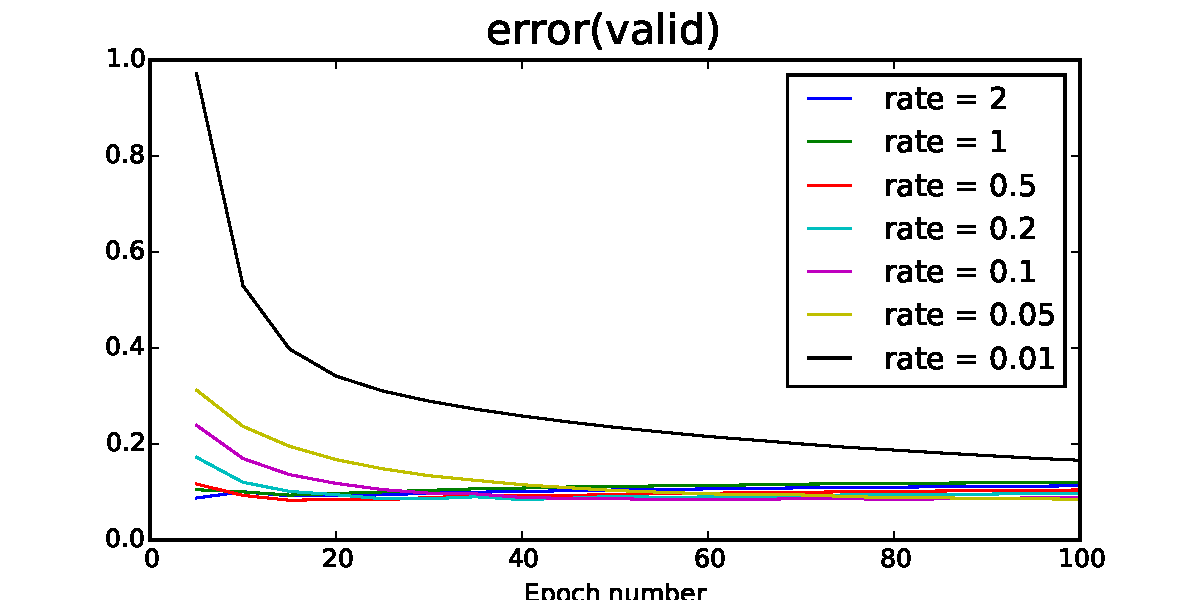
\includegraphics[width=7cm]{Task1/figures/Const_rule_error(valid).pdf}
\end{subfigure}%
\end{figure}
\begin{figure}[h]
\centering
\begin{subfigure}{.5\textwidth}
  \centering
  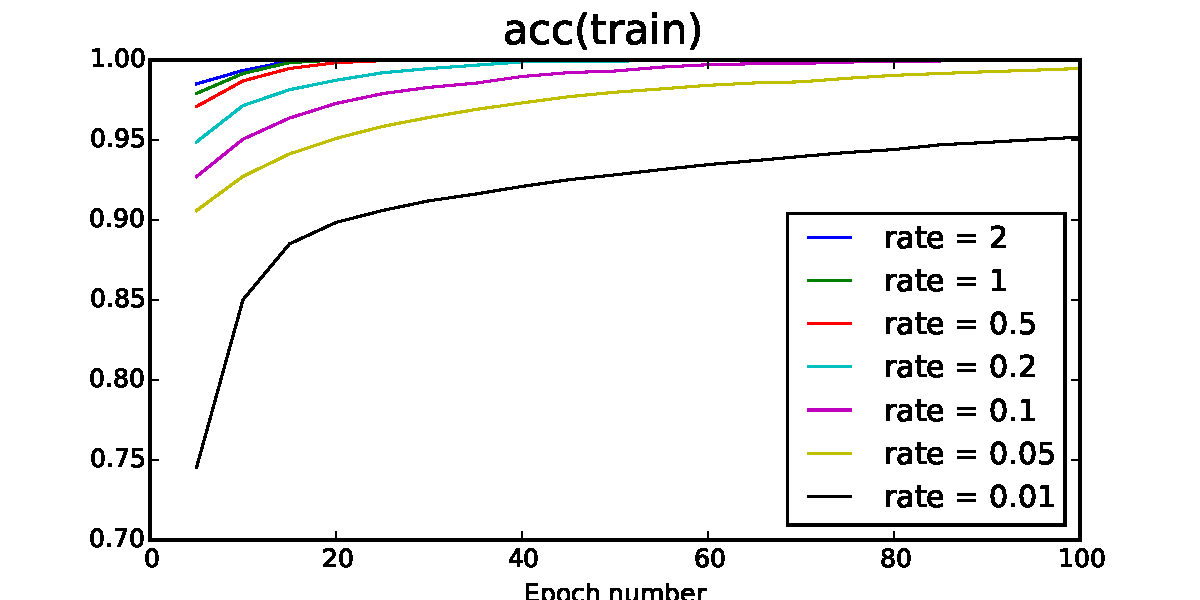
\includegraphics[width=7cm]{Task1/figures/Const_rule_acc(train).pdf}
\end{subfigure}%
\begin{subfigure}{.5\textwidth}
  \centering
  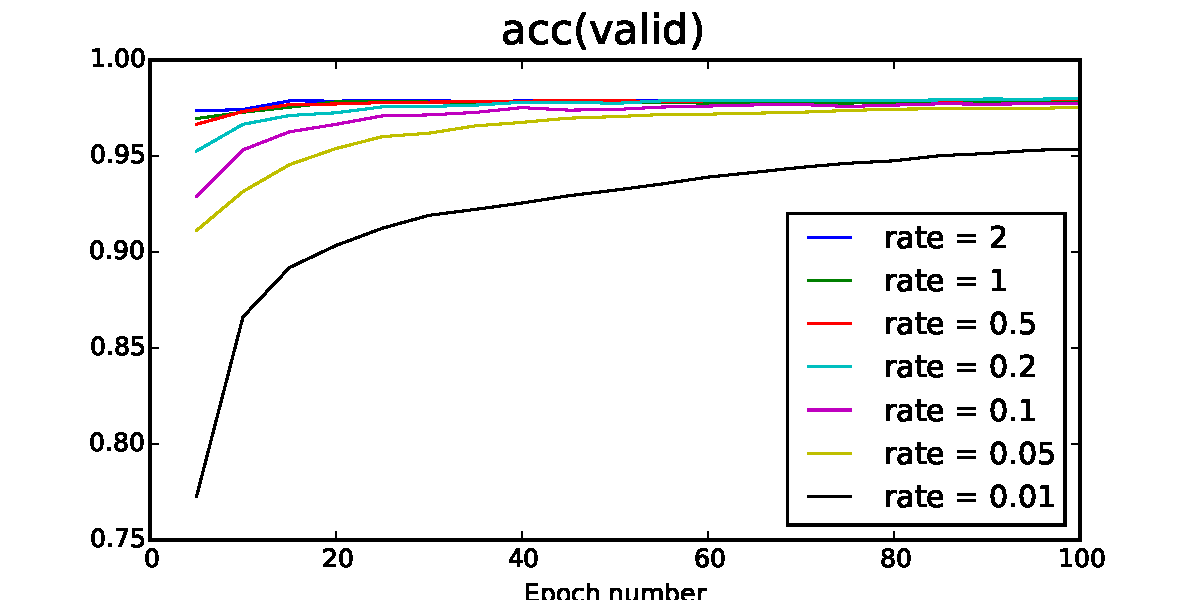
\includegraphics[width=7cm]{Task1/figures/Const_rule_acc(valid).pdf}
\end{subfigure}%
  \caption{Constant learning rate hyperparameter results.}
  \label{fig:const}
\end{figure}

Figure \ref{fig:const} displays effect of different learning rates on error and accuracy. Showing that learning rate of around 0.01 converges the quickest to an accuracy comparable with most other learning rates displayed. The model converges after 20 epochs and from that point it starts being over-fitted to the data. 






\begin{figure}[h]
\centering
\begin{subfigure}{.5\textwidth}
  \centering
  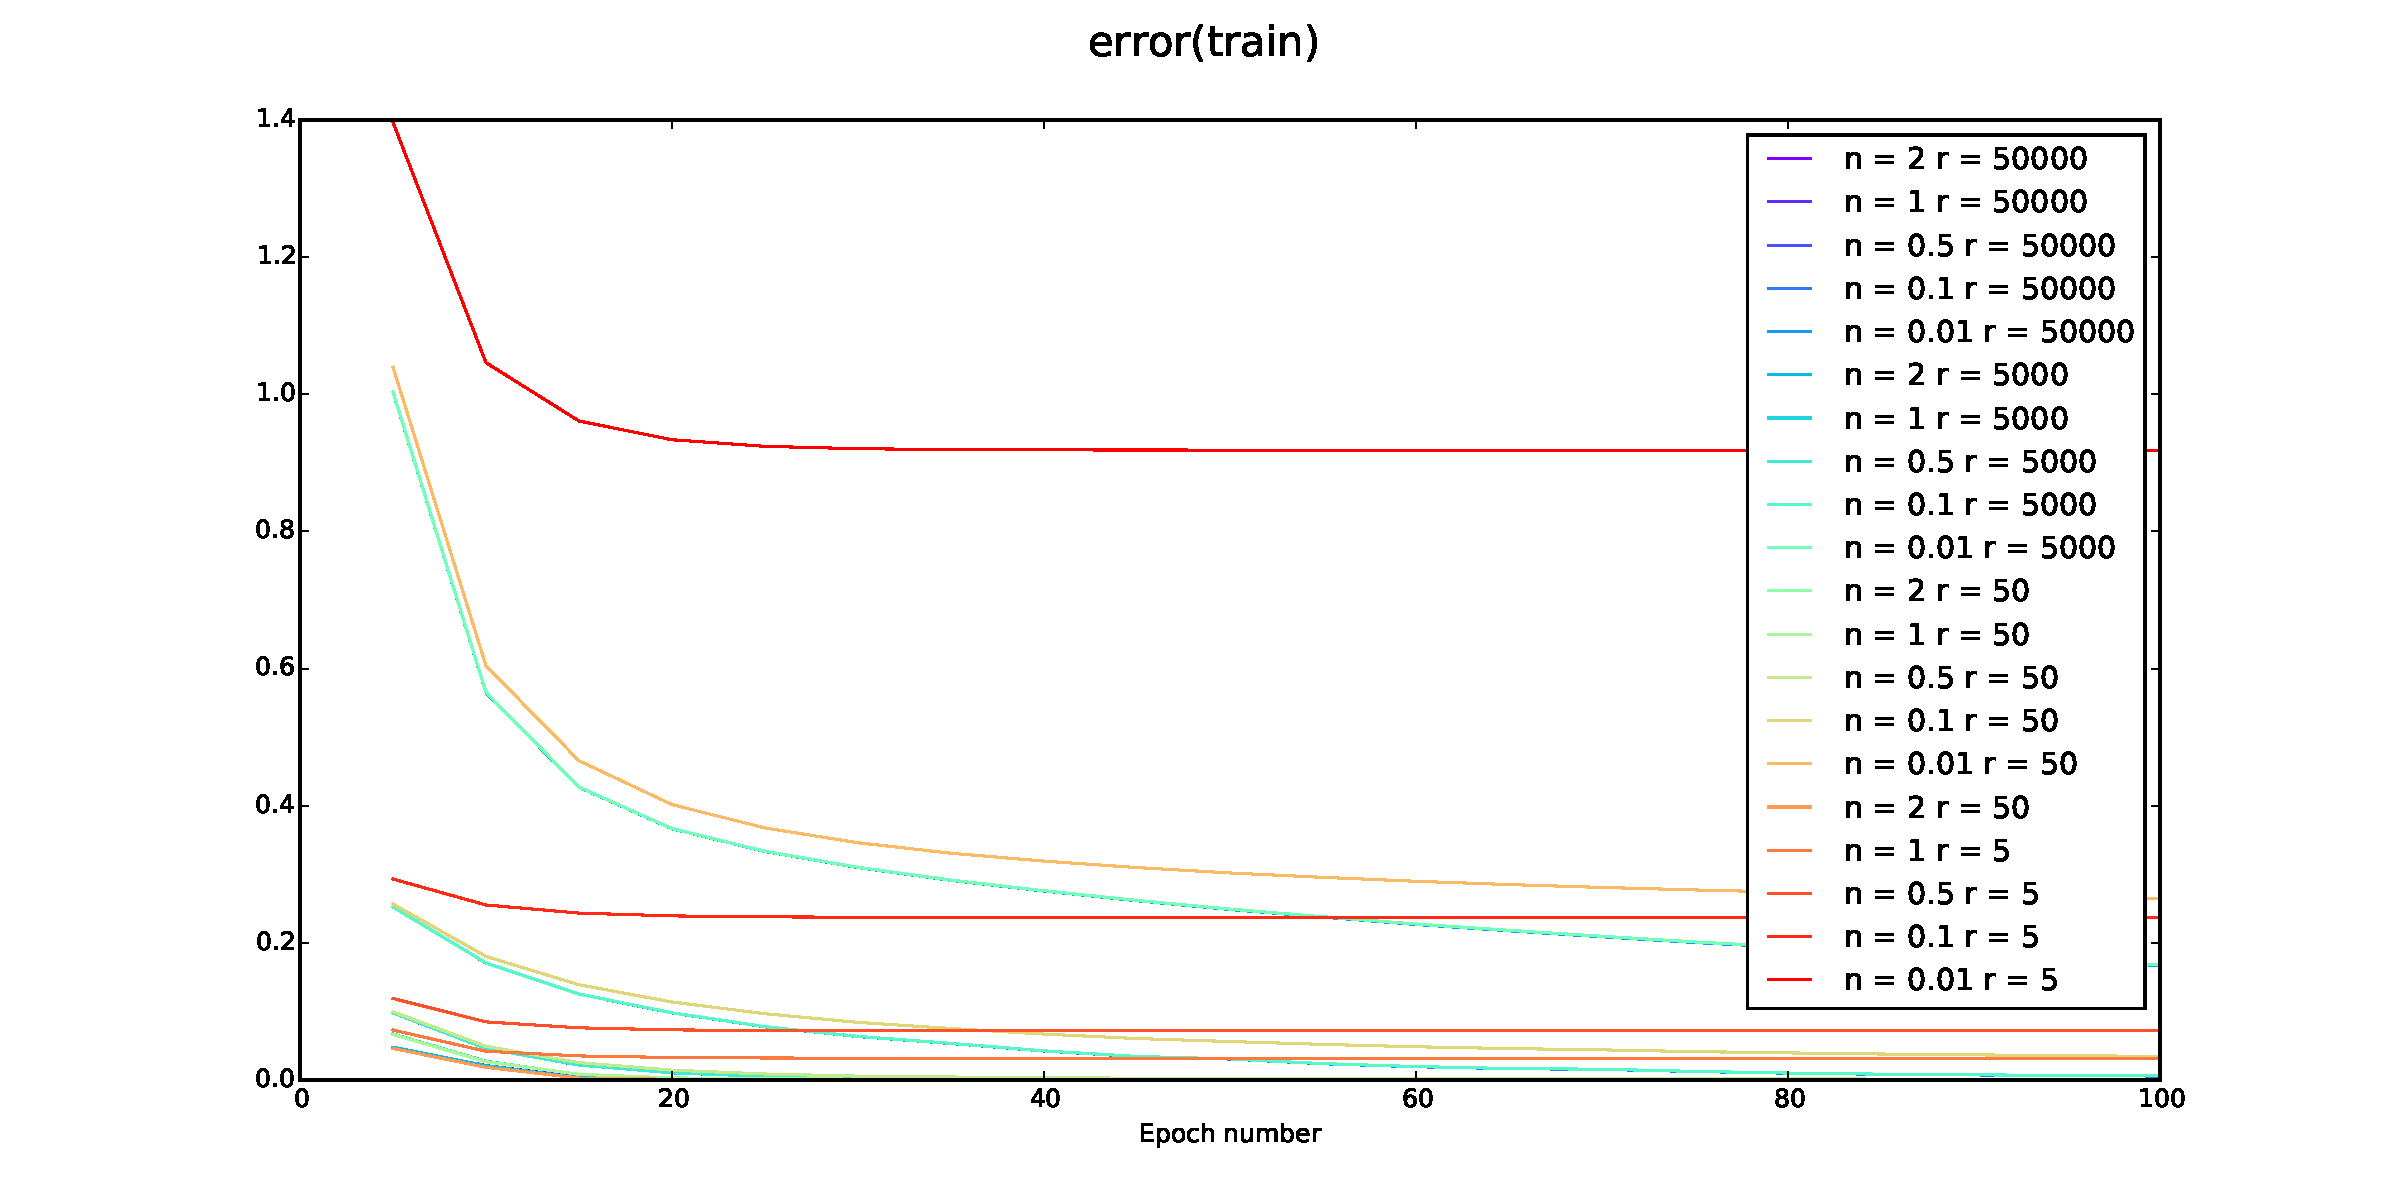
\includegraphics[width=9.1cm]{Task1/figures/Exp_rule_error(train).pdf}
\end{subfigure}%
\begin{subfigure}{.5\textwidth}
  \centering
  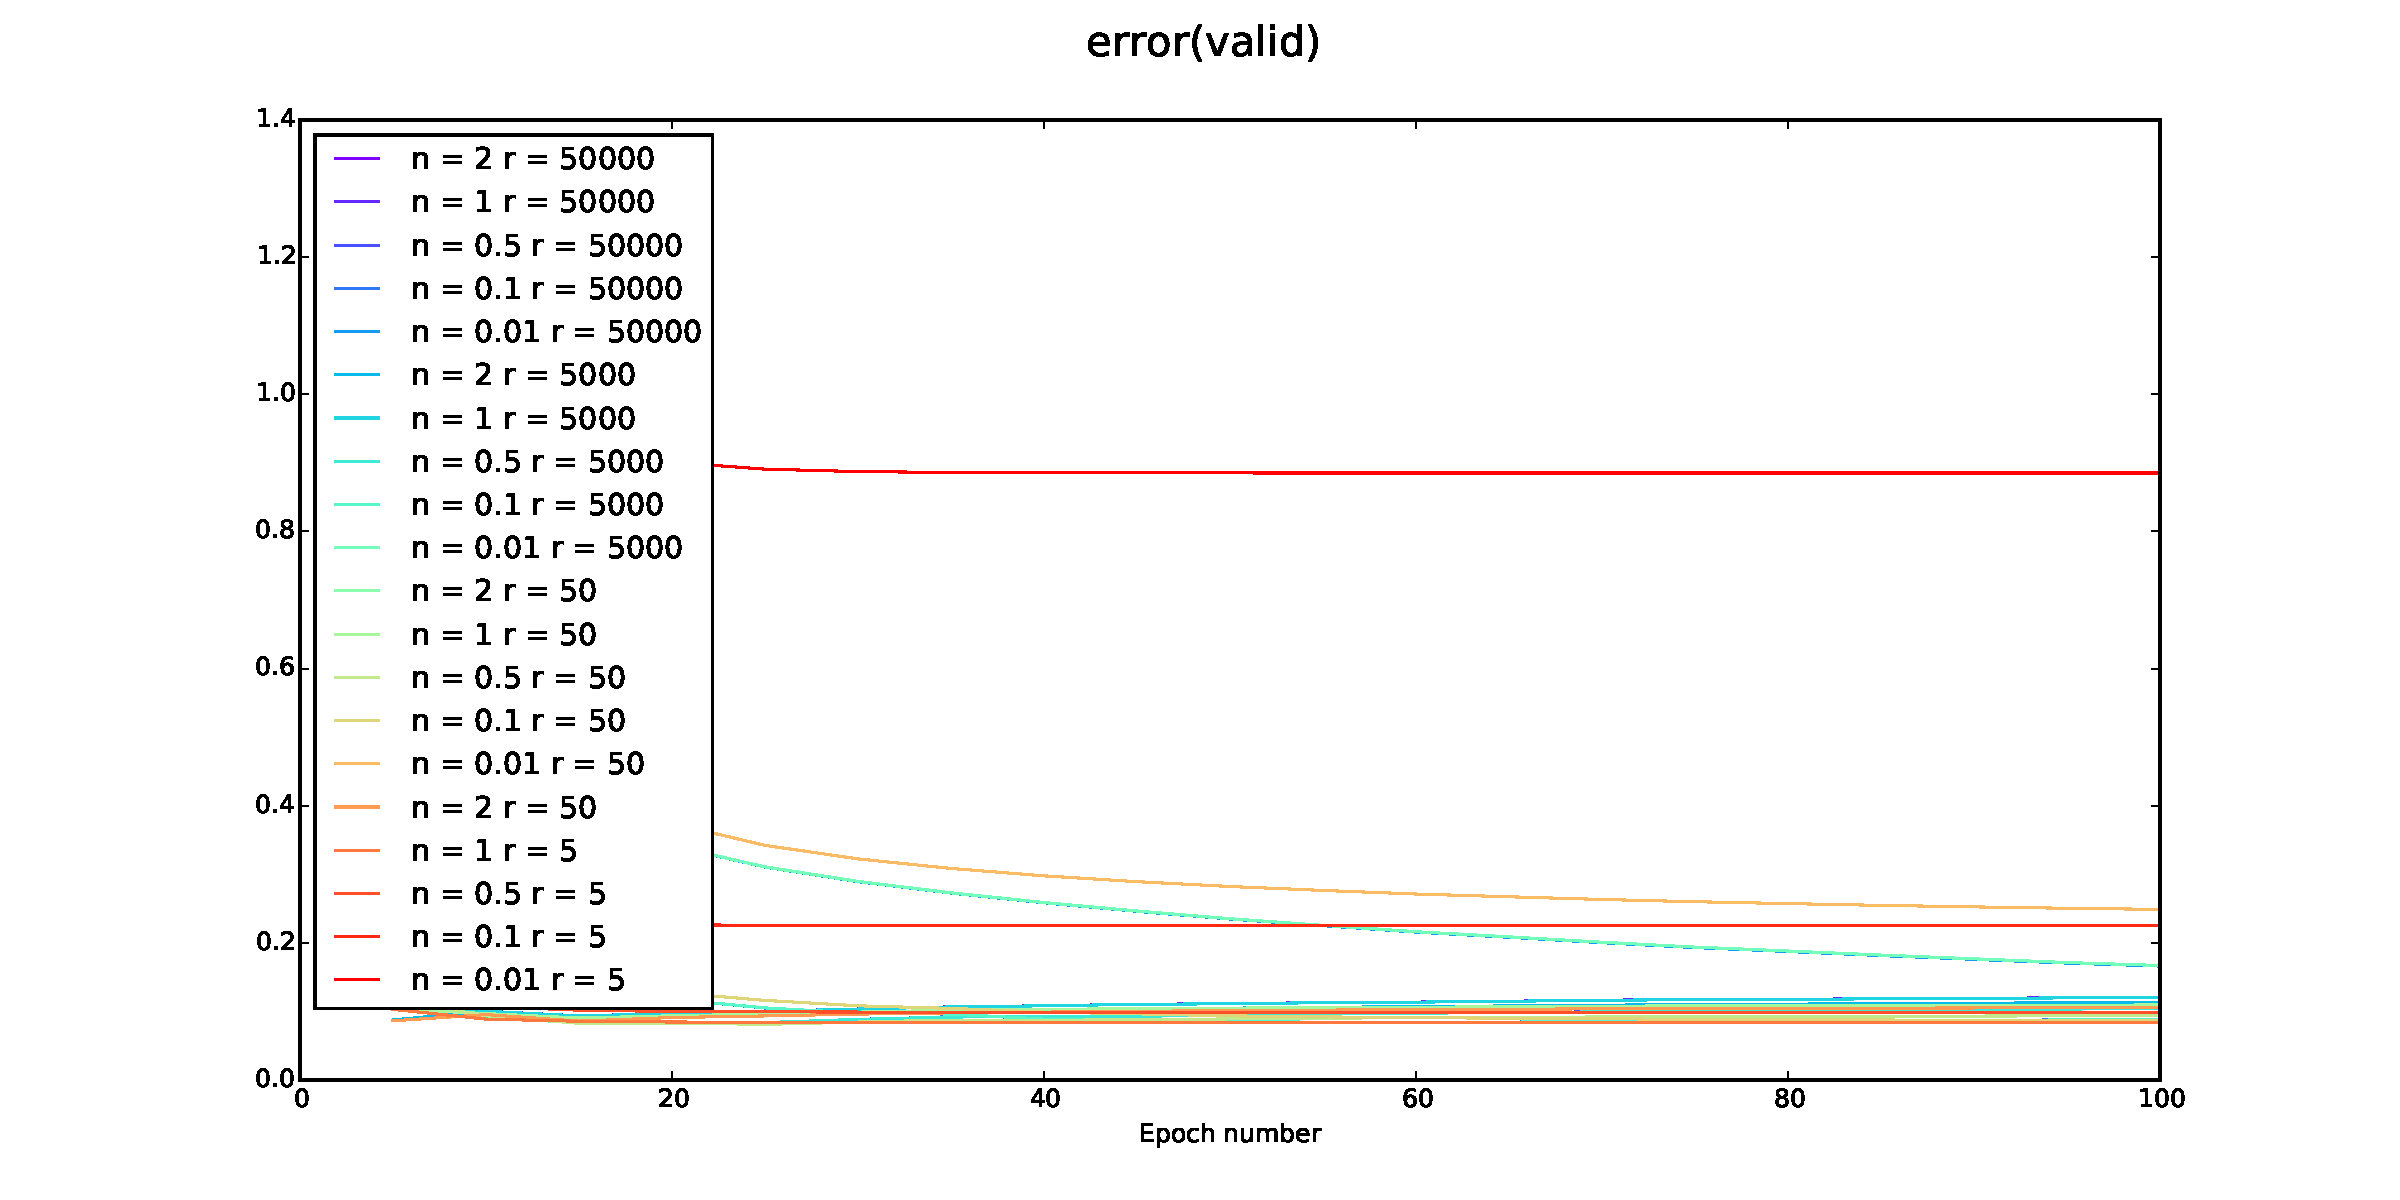
\includegraphics[width=9.1cm]{Task1/figures/Exp_rule_error(valid).pdf}
\end{subfigure}%
\end{figure}
\begin{figure}[h]
\centering
\begin{subfigure}{.5\textwidth}
  \centering
  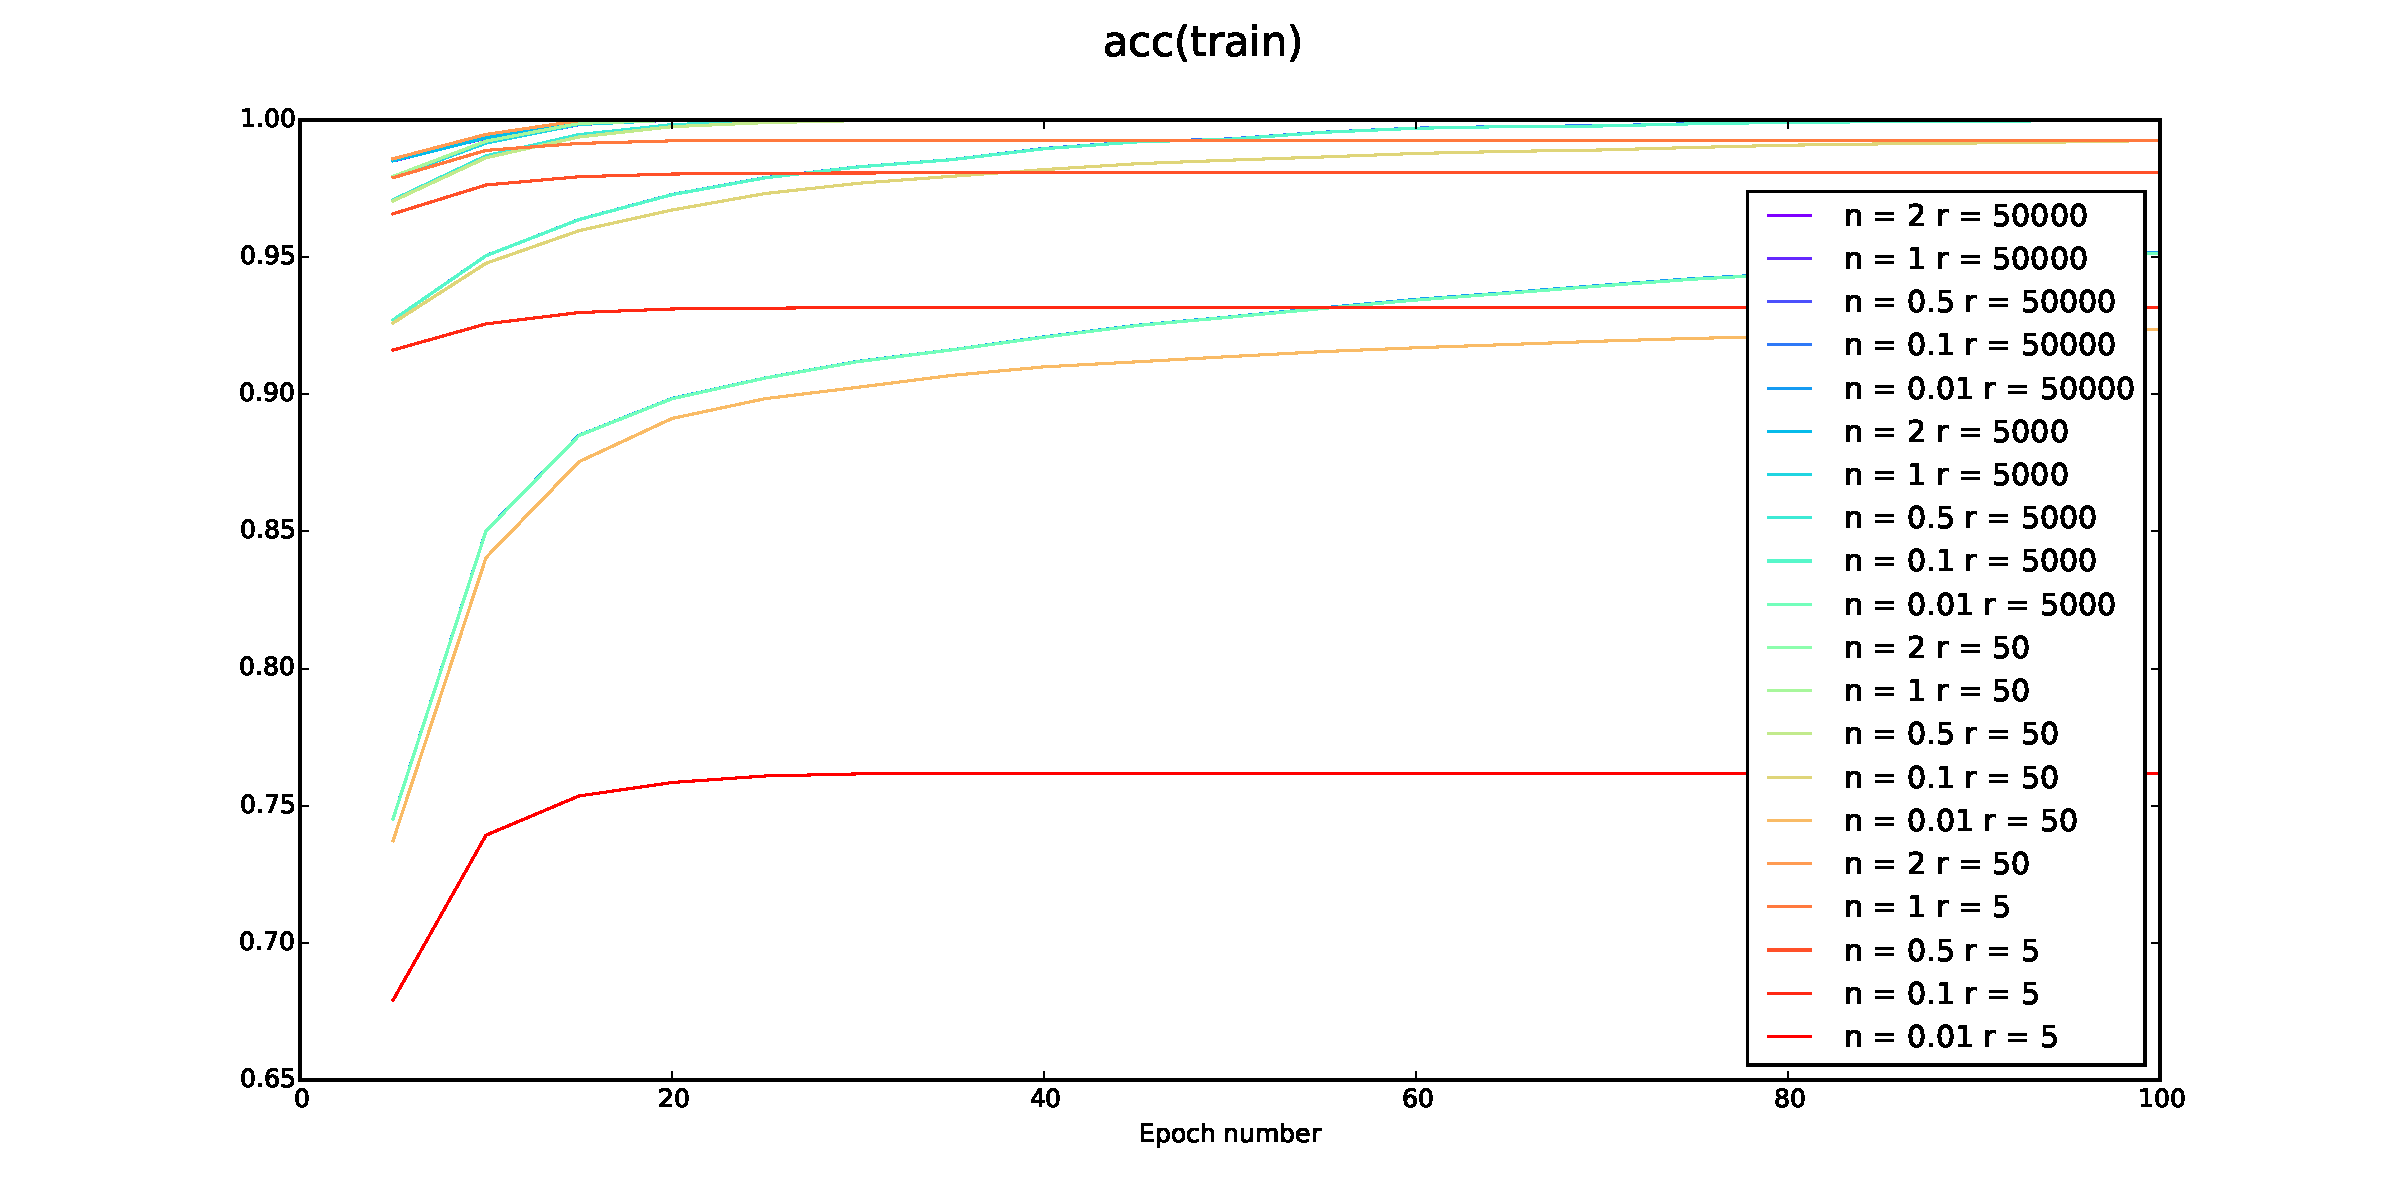
\includegraphics[width=9.1cm]{Task1/figures/Exp_rule_acc(train).pdf}
\end{subfigure}%
\begin{subfigure}{.5\textwidth}
  \centering
  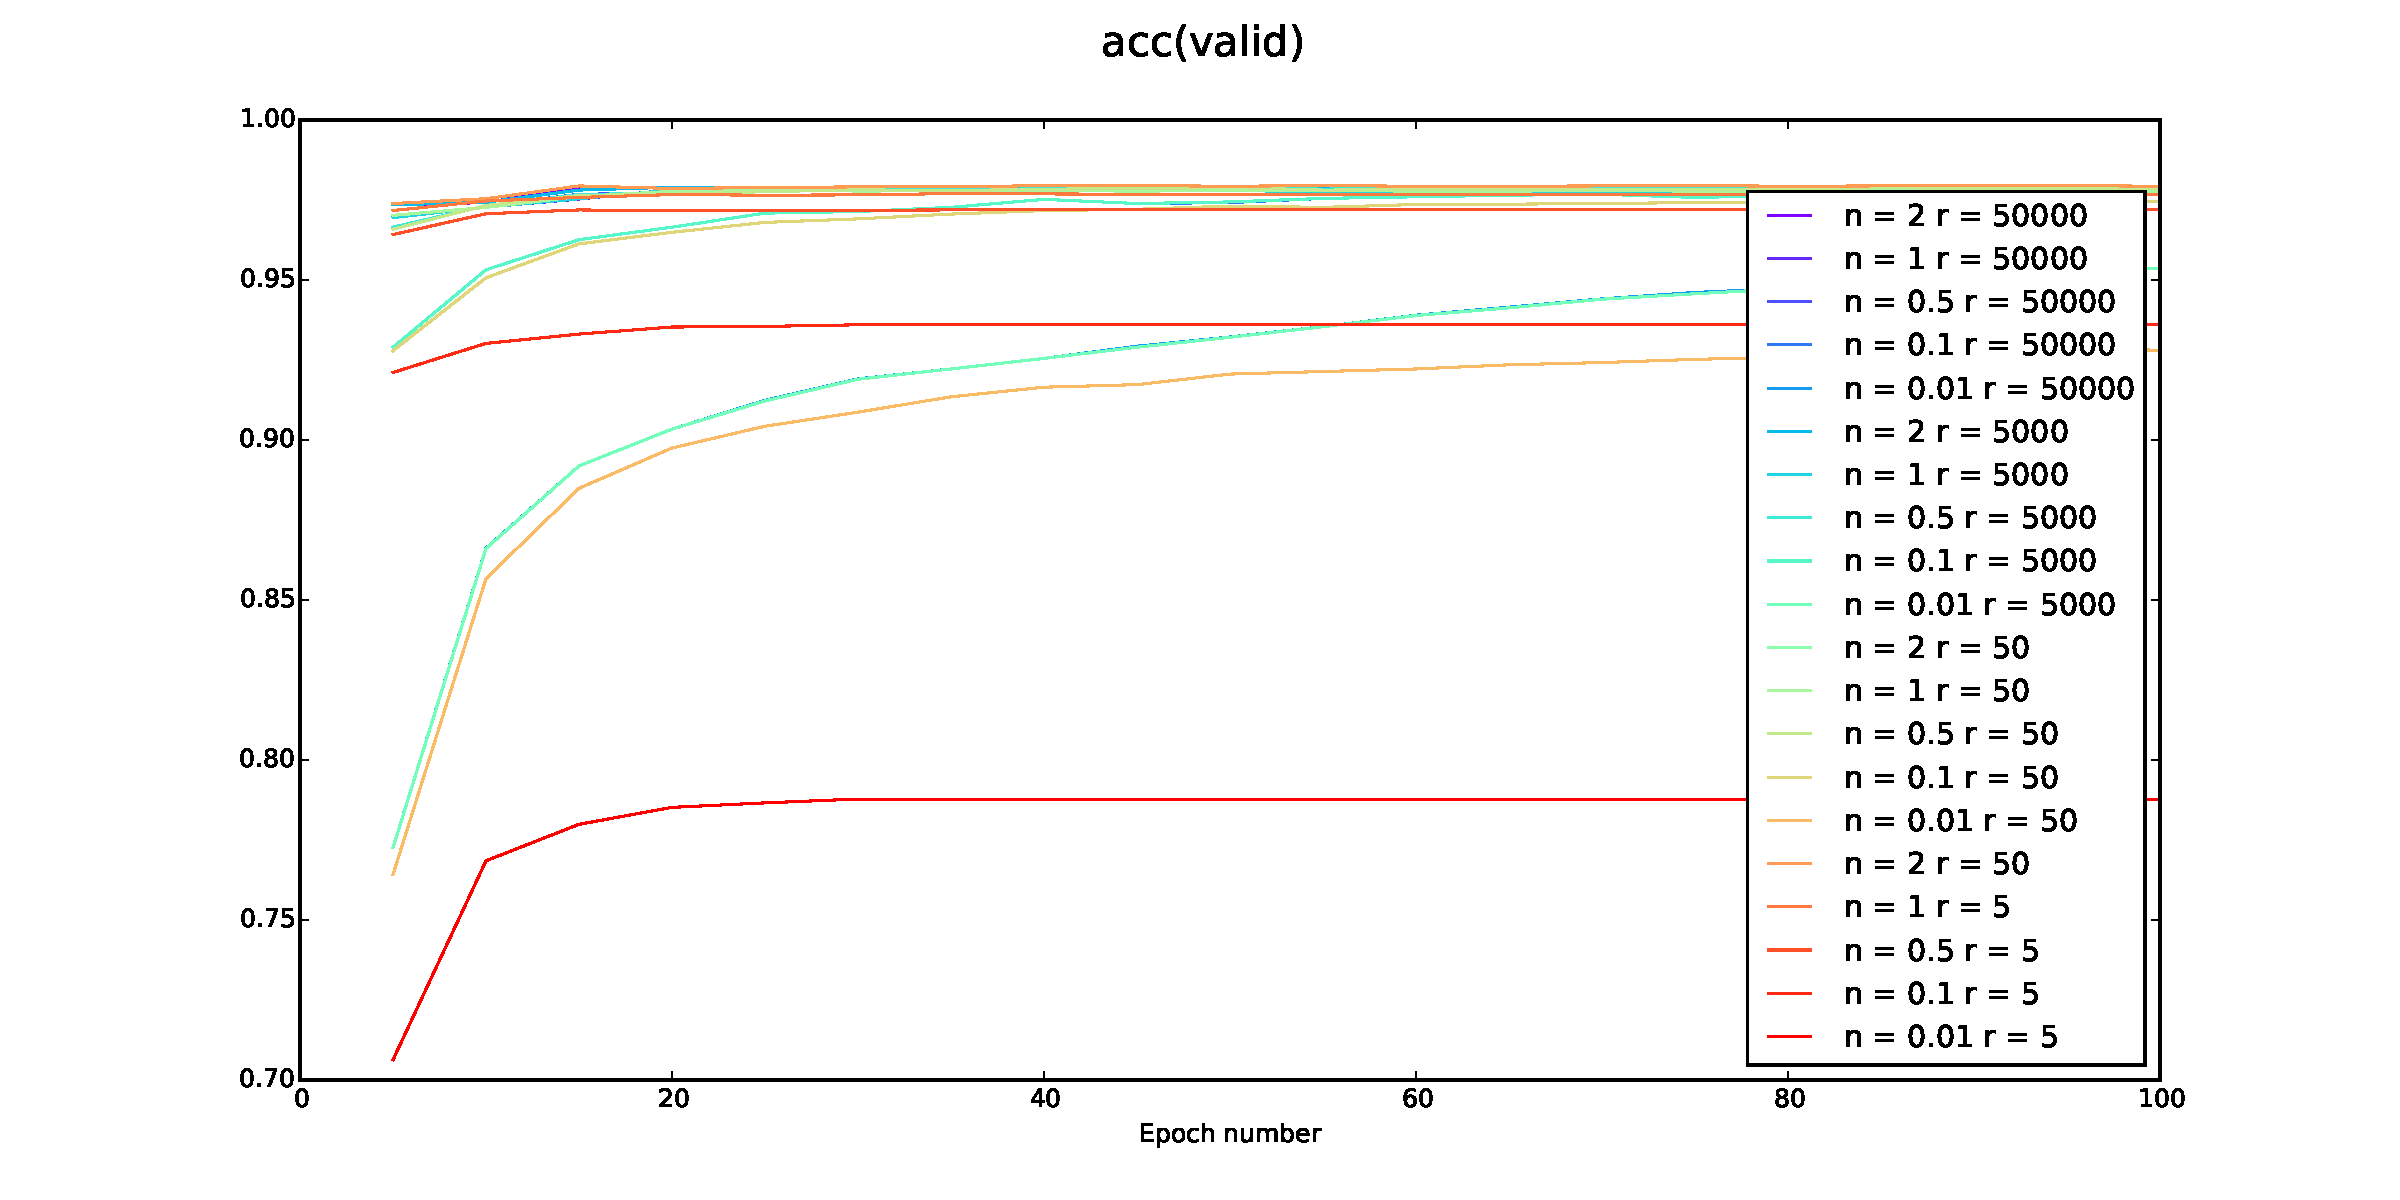
\includegraphics[width=9.1cm]{Task1/figures/Exp_rule_acc(valid).pdf}
\end{subfigure}%
  \caption{Exponential learning rate hyperparameter results.}
  \label{fig:exp}
\end{figure}

Figure \ref{fig:exp} displays the effect of different hyperparameters on the exponential learning rate. Parameter r dictates how quickly the rate decays and to which final value. Two extremes can happen: one the model with stop learning after a small number of epochs (small r), or the rate does not really decay (large r). Parameter n scales these learning rate decays which r dictates. 



\begin{figure}[h]
\centering
\begin{subfigure}{.5\textwidth}
\centering
\begin{tabular}[h]{| c | c |}
\hline
Learning rate &  Accuracy(valid) \\
\hline 
2 & 0.978   \\
\hline
1 & 0.977   \\
\hline
0.5 & 0.979   \\
\hline
0.2 & 0.98   \\
\hline
0.1 & 0.977   \\
\hline
0.05 & 0.975   \\
\hline
0.01 & 0.953   \\
\hline
\end{tabular}
\end{subfigure}%
\begin{subfigure}{.5\textwidth}

\centering
\begin{tabular}[h]{| c | c | c |}
\hline
n & r & Accuracy(valid) \\
\hline
2 & 50000 & 0.979 \\
\hline
1 & 50000 & 0.9779 \\
\hline
0.5 & 50000 & 0.9793 \\
\hline
0.1 & 50000 & 0.9772 \\
\hline
0.01 & 50000 & 0.9536 \\
\hline
2 & 5000 & 0.9785 \\
\hline
1 & 5000 & 0.978 \\
\hline
0.5 & 5000 & 0.9792 \\
\hline
0.1 & 5000 & 0.9772 \\
\hline
0.01 & 5000 & 0.9536 \\
\hline
2 & 50 & 0.9793 \\
\hline
1 & 50 & 0.9777 \\
\hline
0.5 & 50 & 0.9785 \\
\hline
0.1 & 50 & 0.9745 \\
\hline
0.01 & 50 & 0.9281 \\
\hline
2 & 50 & 0.9793 \\
\hline
1 & 5 & 0.9768 \\
\hline
0.5 & 5 & 0.9719 \\
\hline
0.1 & 5 & 0.9362 \\
\hline
0.01 & 5 & 0.7878 \\
\hline
\end{tabular}
\end{subfigure}%

  \caption{Comparison of Constant and Exponential learning rates accuracies on the validation set.}
  \label{fig:task1_table}
\end{figure}

Comparing the performance with the constant learning rate, the exponential rate converges as quickly as constant on the optimal parameters and in general faster. It also is a bit less over-fitted thanks to the decay.

\section*{Task 2 - Momentum learning rule }
The second section introduces momentum or velocity to the gradient descent. This allows the model to overcome shallow local minima. The model will try to keep a more stable descent direction and will be less thrown off by possibly wrong direction introduced by the batches. The momentum learning rule relies on a coefficient alpha of how much memory it keeps of the past direction. This section investigates how different values of alpha influence the training and performance. The learning rate used is 0.2 as it performed well in the past tests.

\begin{figure}[h]
\centering
\begin{subfigure}{.5\textwidth}
  \centering
  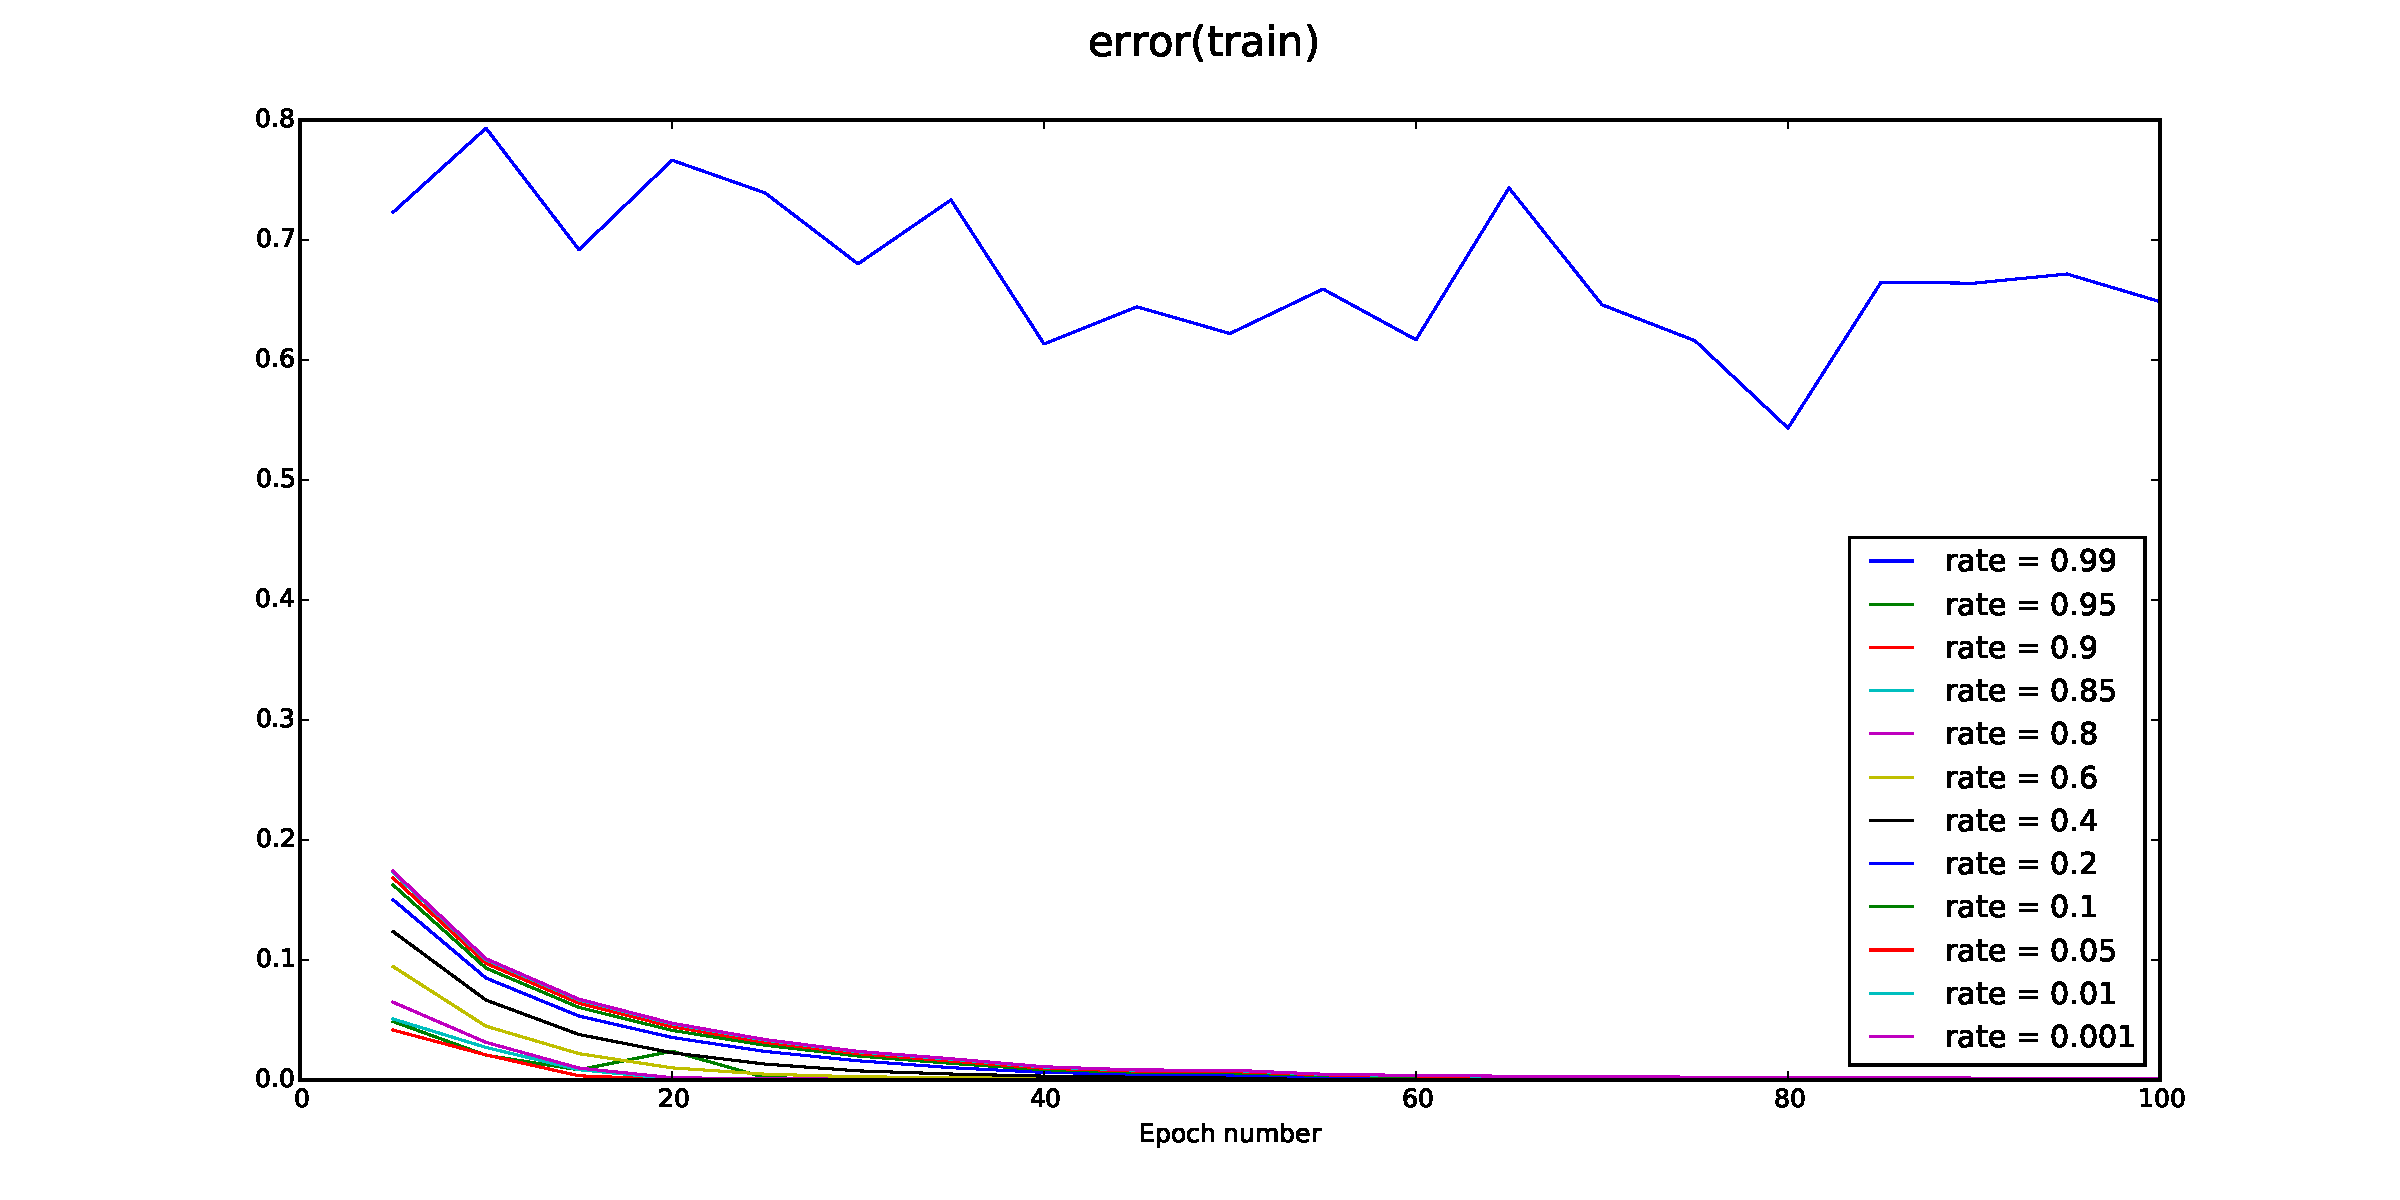
\includegraphics[width=9.1cm]{Task2/figures/Only_mome_error(train).pdf}
\end{subfigure}%
\begin{subfigure}{.5\textwidth}
  \centering
  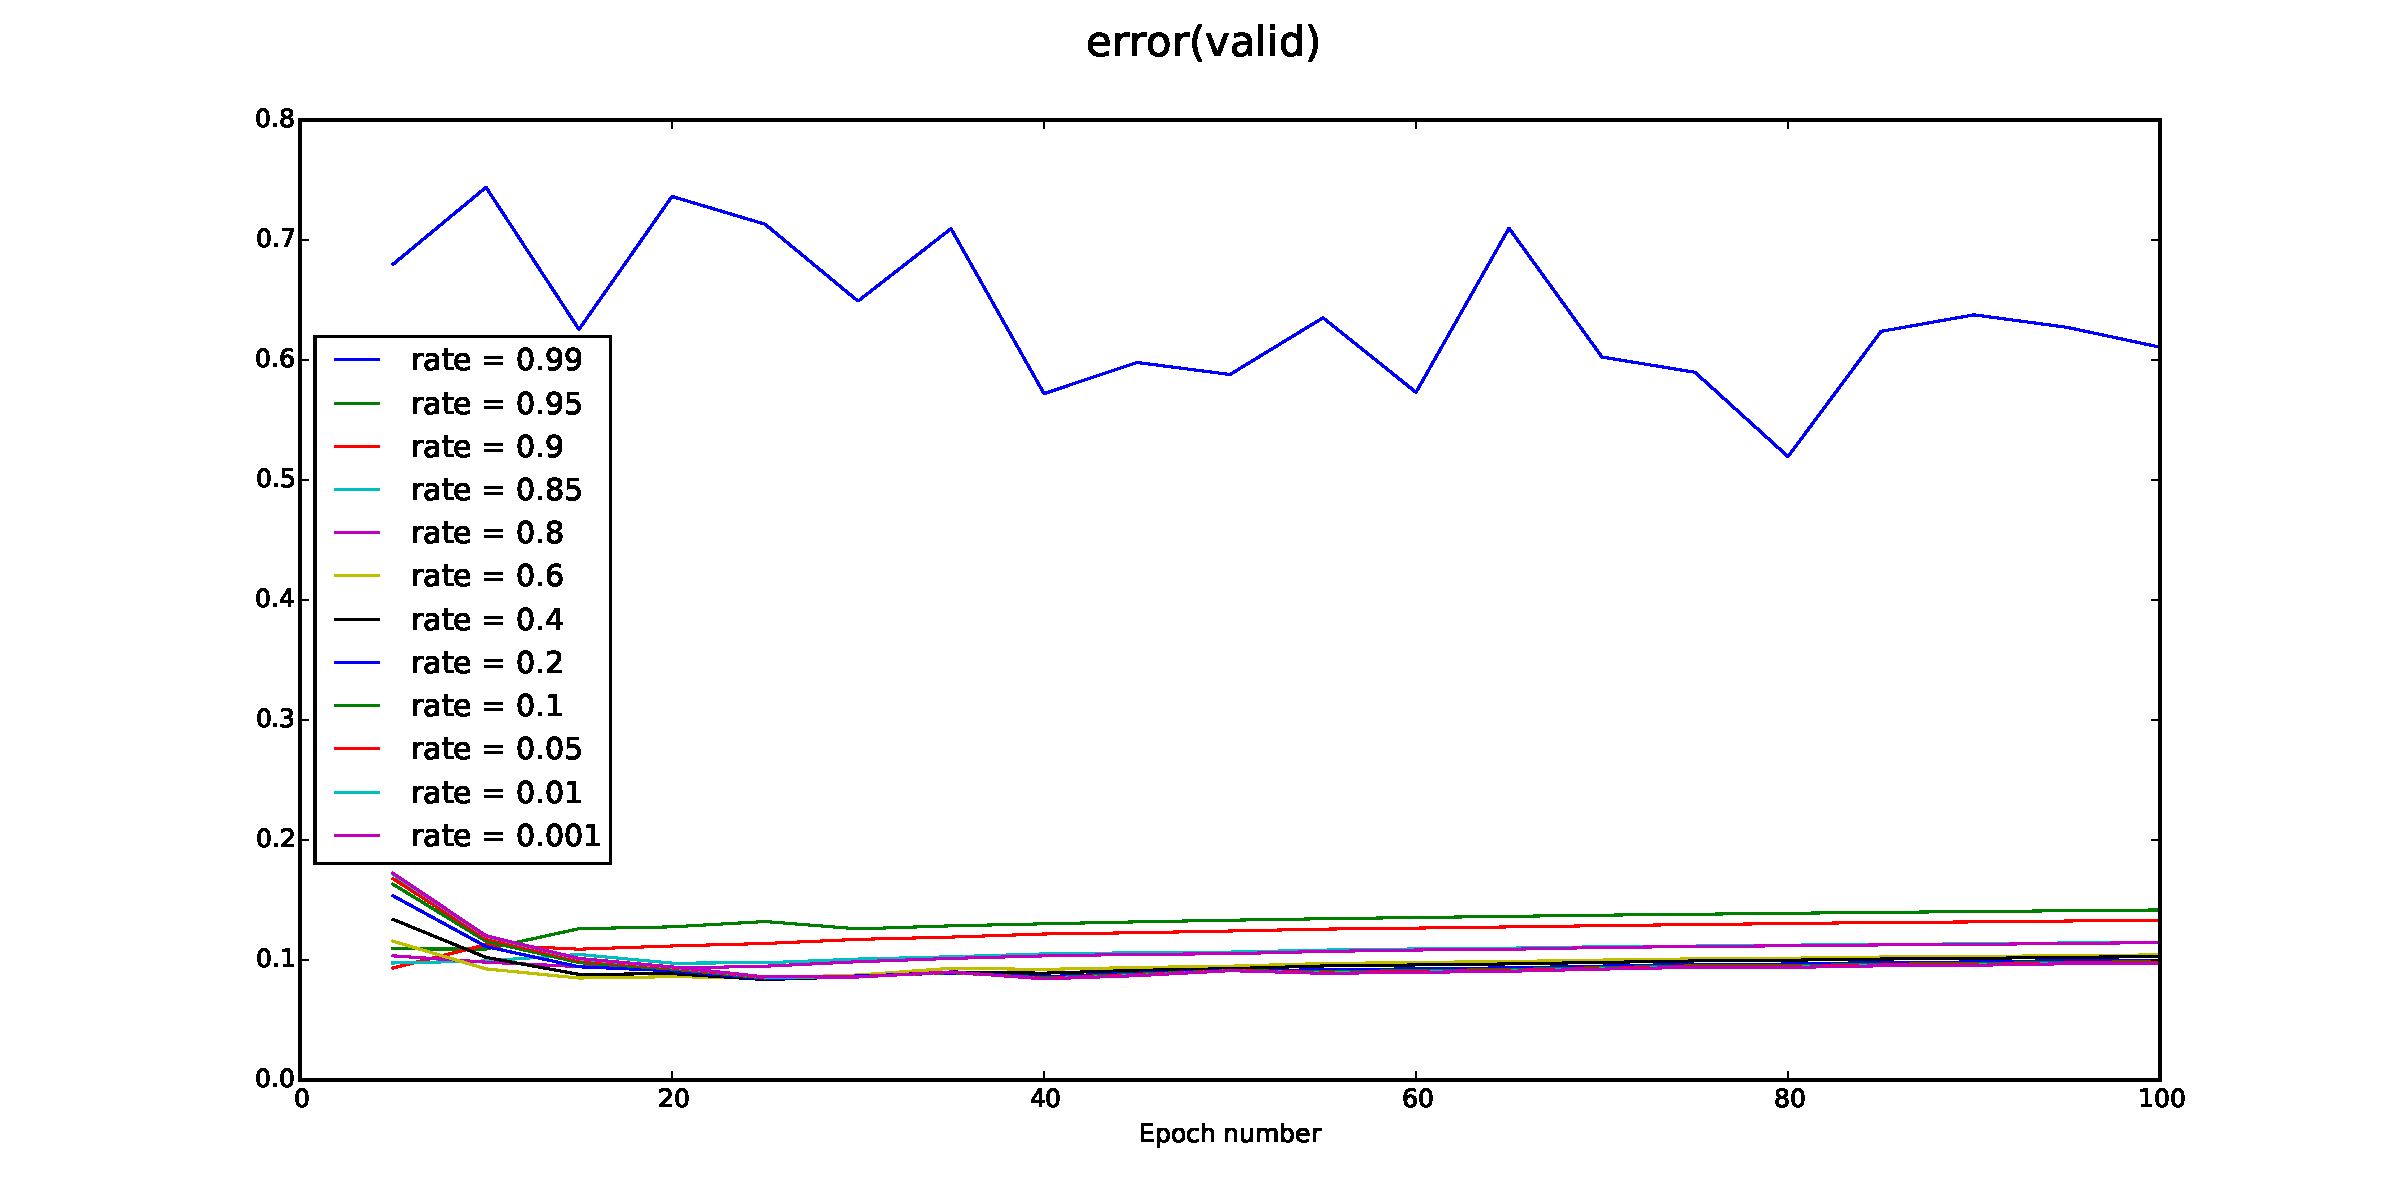
\includegraphics[width=9.1cm]{Task2/figures/Only_mome_error(valid).pdf}
\end{subfigure}%
\end{figure}
\begin{figure}[h]
\centering
\begin{subfigure}{.5\textwidth}
  \centering
  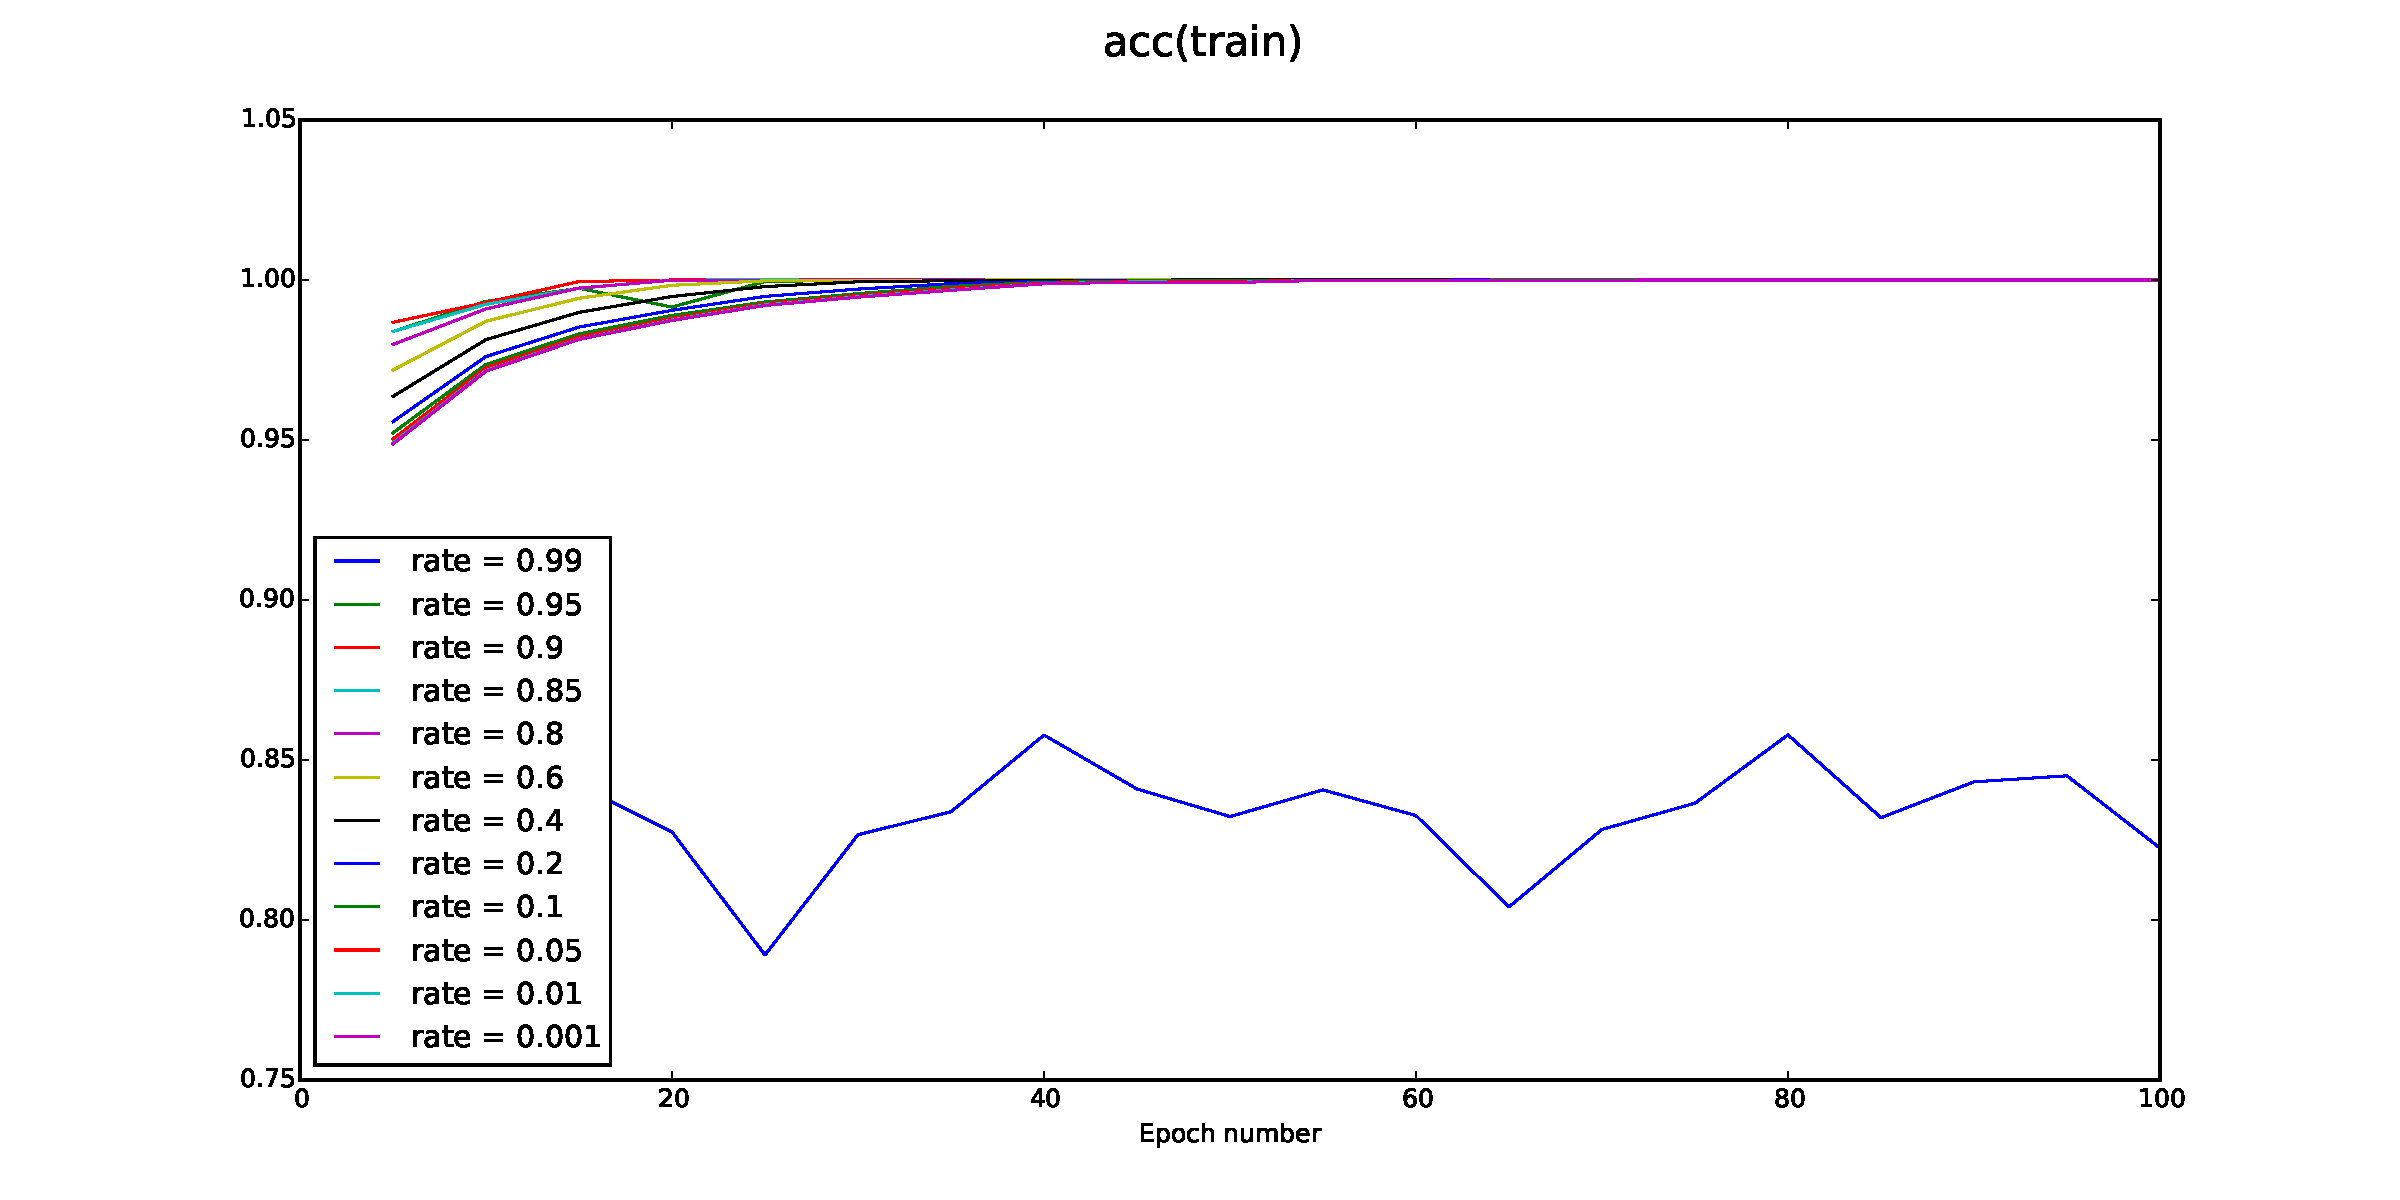
\includegraphics[width=9.1cm]{Task2/figures/Only_mome_acc(train).pdf}
\end{subfigure}%
\begin{subfigure}{.5\textwidth}
  \centering
  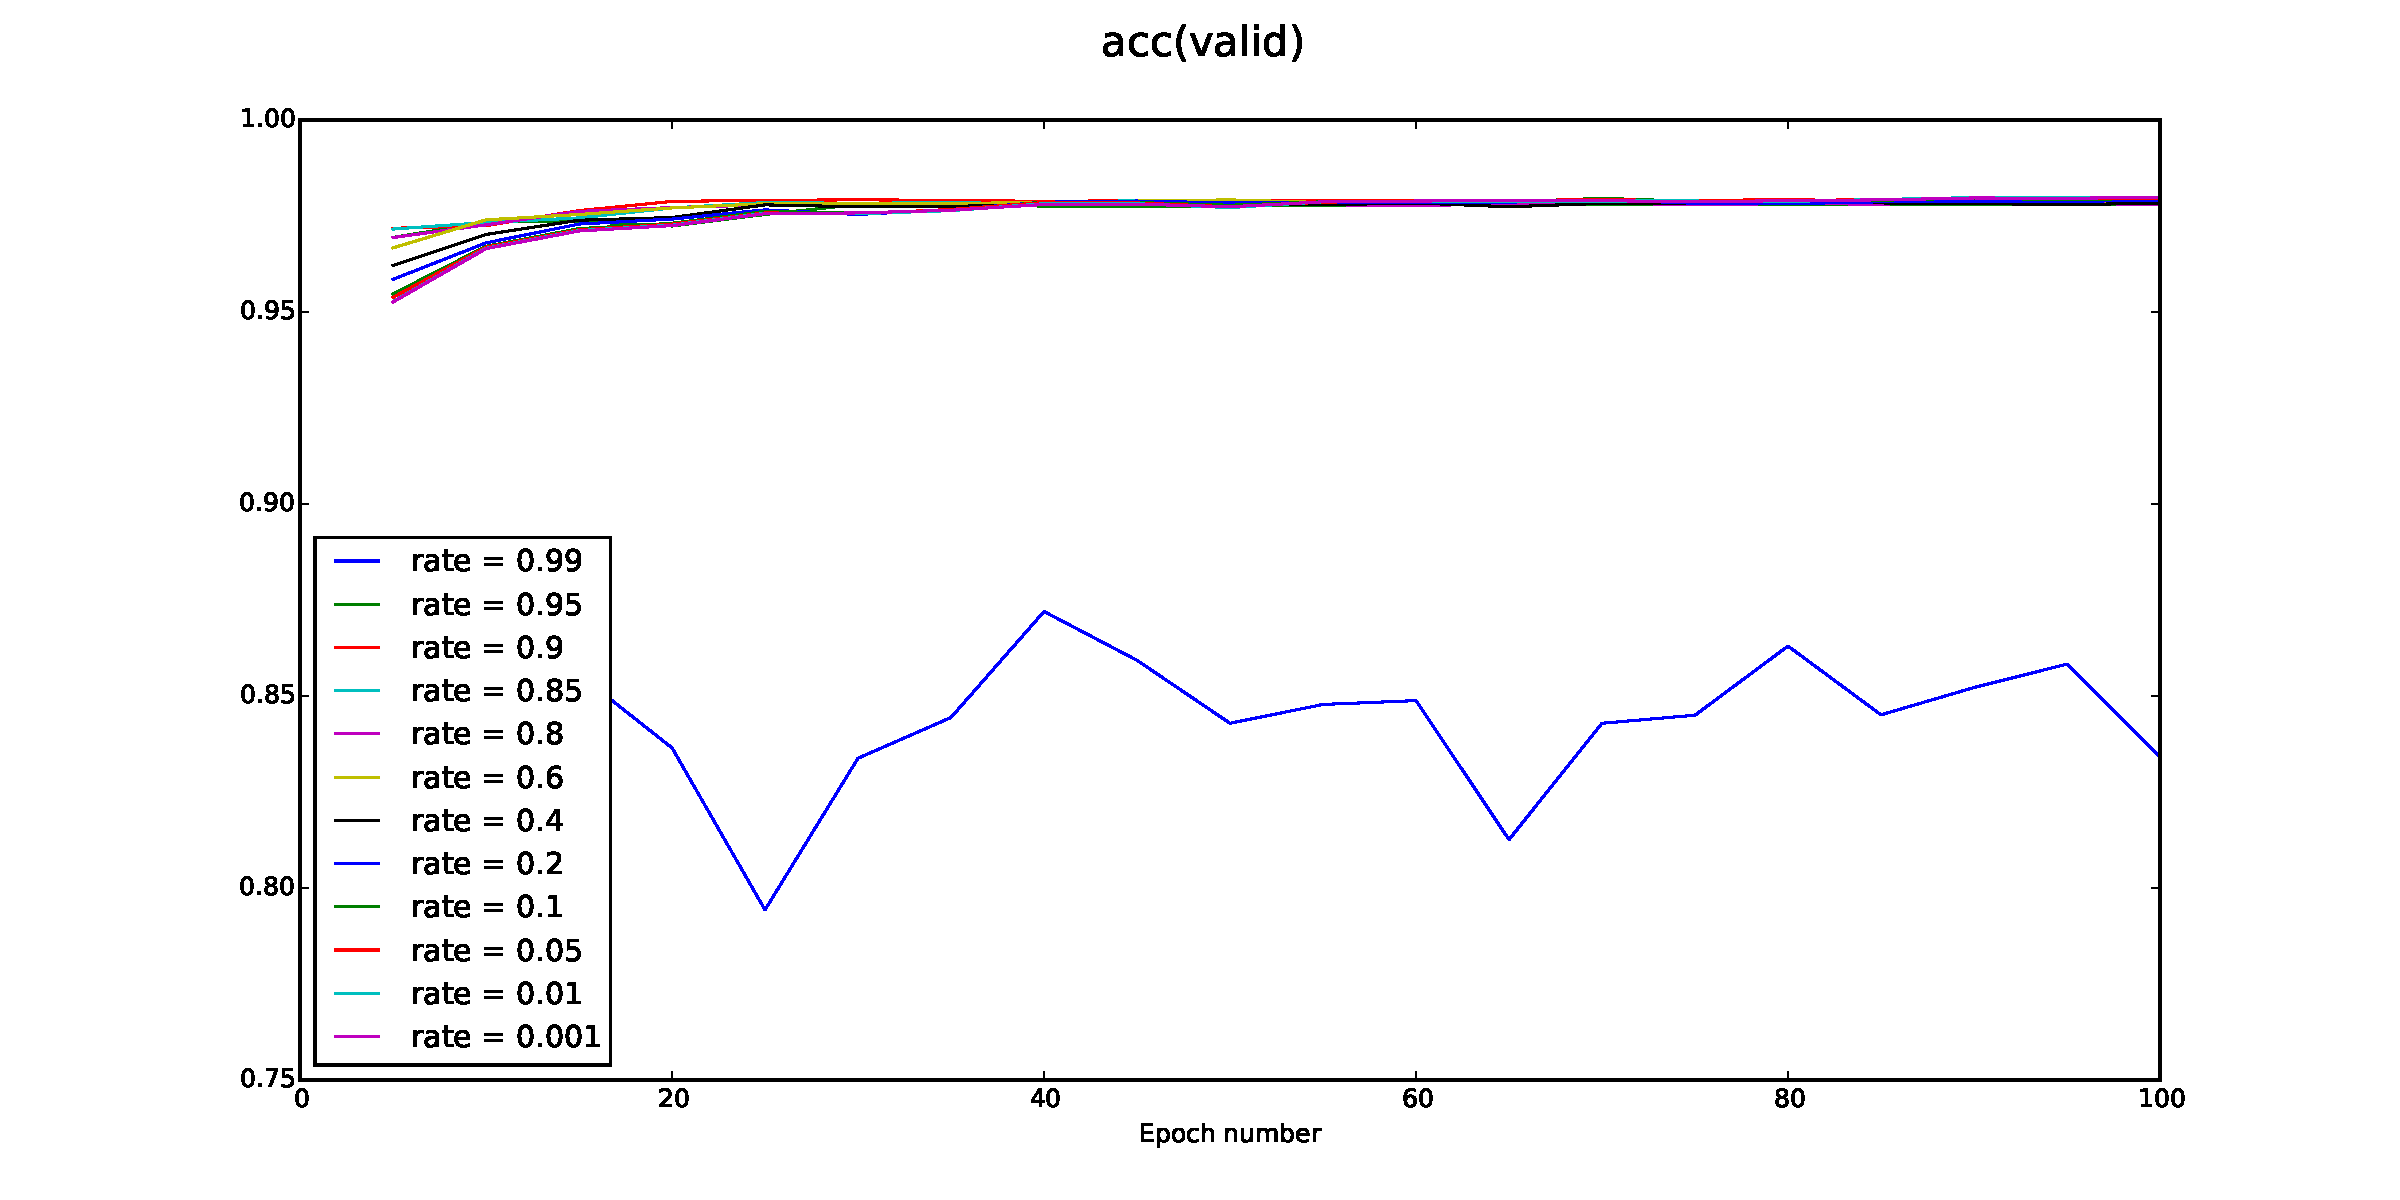
\includegraphics[width=9.1cm]{Task2/figures/Only_mome_acc(valid).pdf}
\end{subfigure}%
  \caption{Momentum learning rule hyperparameter results.}
  \label{fig:only_mome}
\end{figure}

Figure \ref{fig:only_mome} displays effect of the alhpa hyperparameter on training and final performance. It shows that the model performs the best with alpha of 0.9 a generally accepted value. The value alhpa affects the speed of convergence. This model achieves similar performance to the baseline model for the final results, but the speed of convergence should be in general improved.

Next, this section investigates how changing the momentum over time changes the performance of our model. The idea being similar to exponential decay in the last section, only from the opposite side. The goal is to start with a small value of alhpa and end with a large one at the end of training, due to larger variances in gradient at the start compared with the end.
\[ a(t) = a*(1-y/{(t-tau)})\] 

\begin{figure}[h]
\centering
\begin{subfigure}{.5\textwidth}
  \centering
  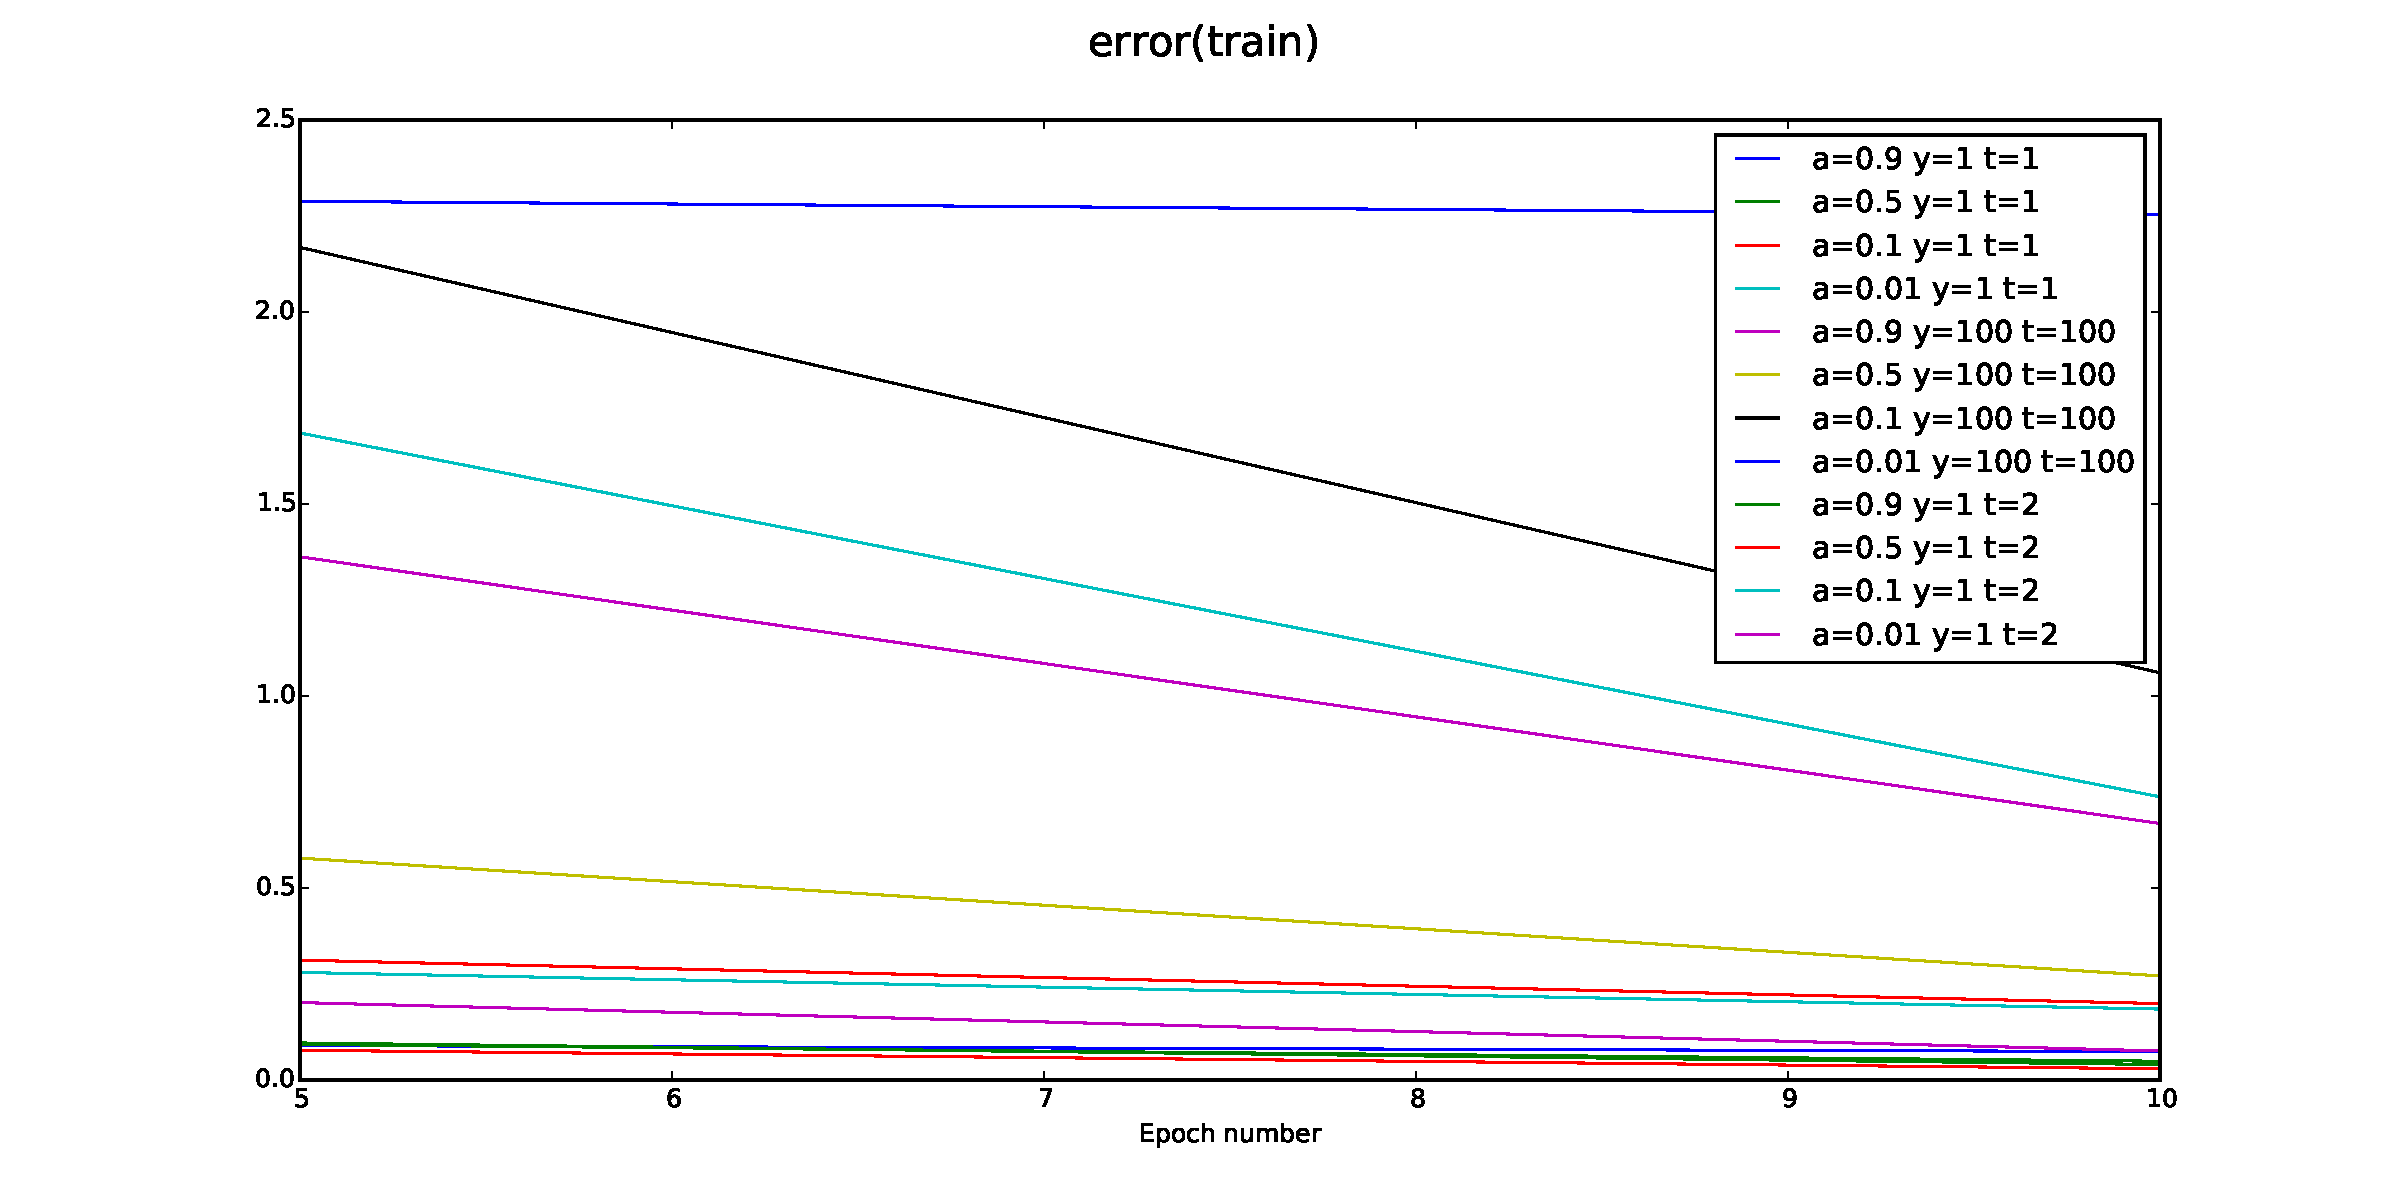
\includegraphics[width=9.1cm]{Task2/figures/Mome_var_error(train).pdf}
\end{subfigure}%
\begin{subfigure}{.5\textwidth}
  \centering
  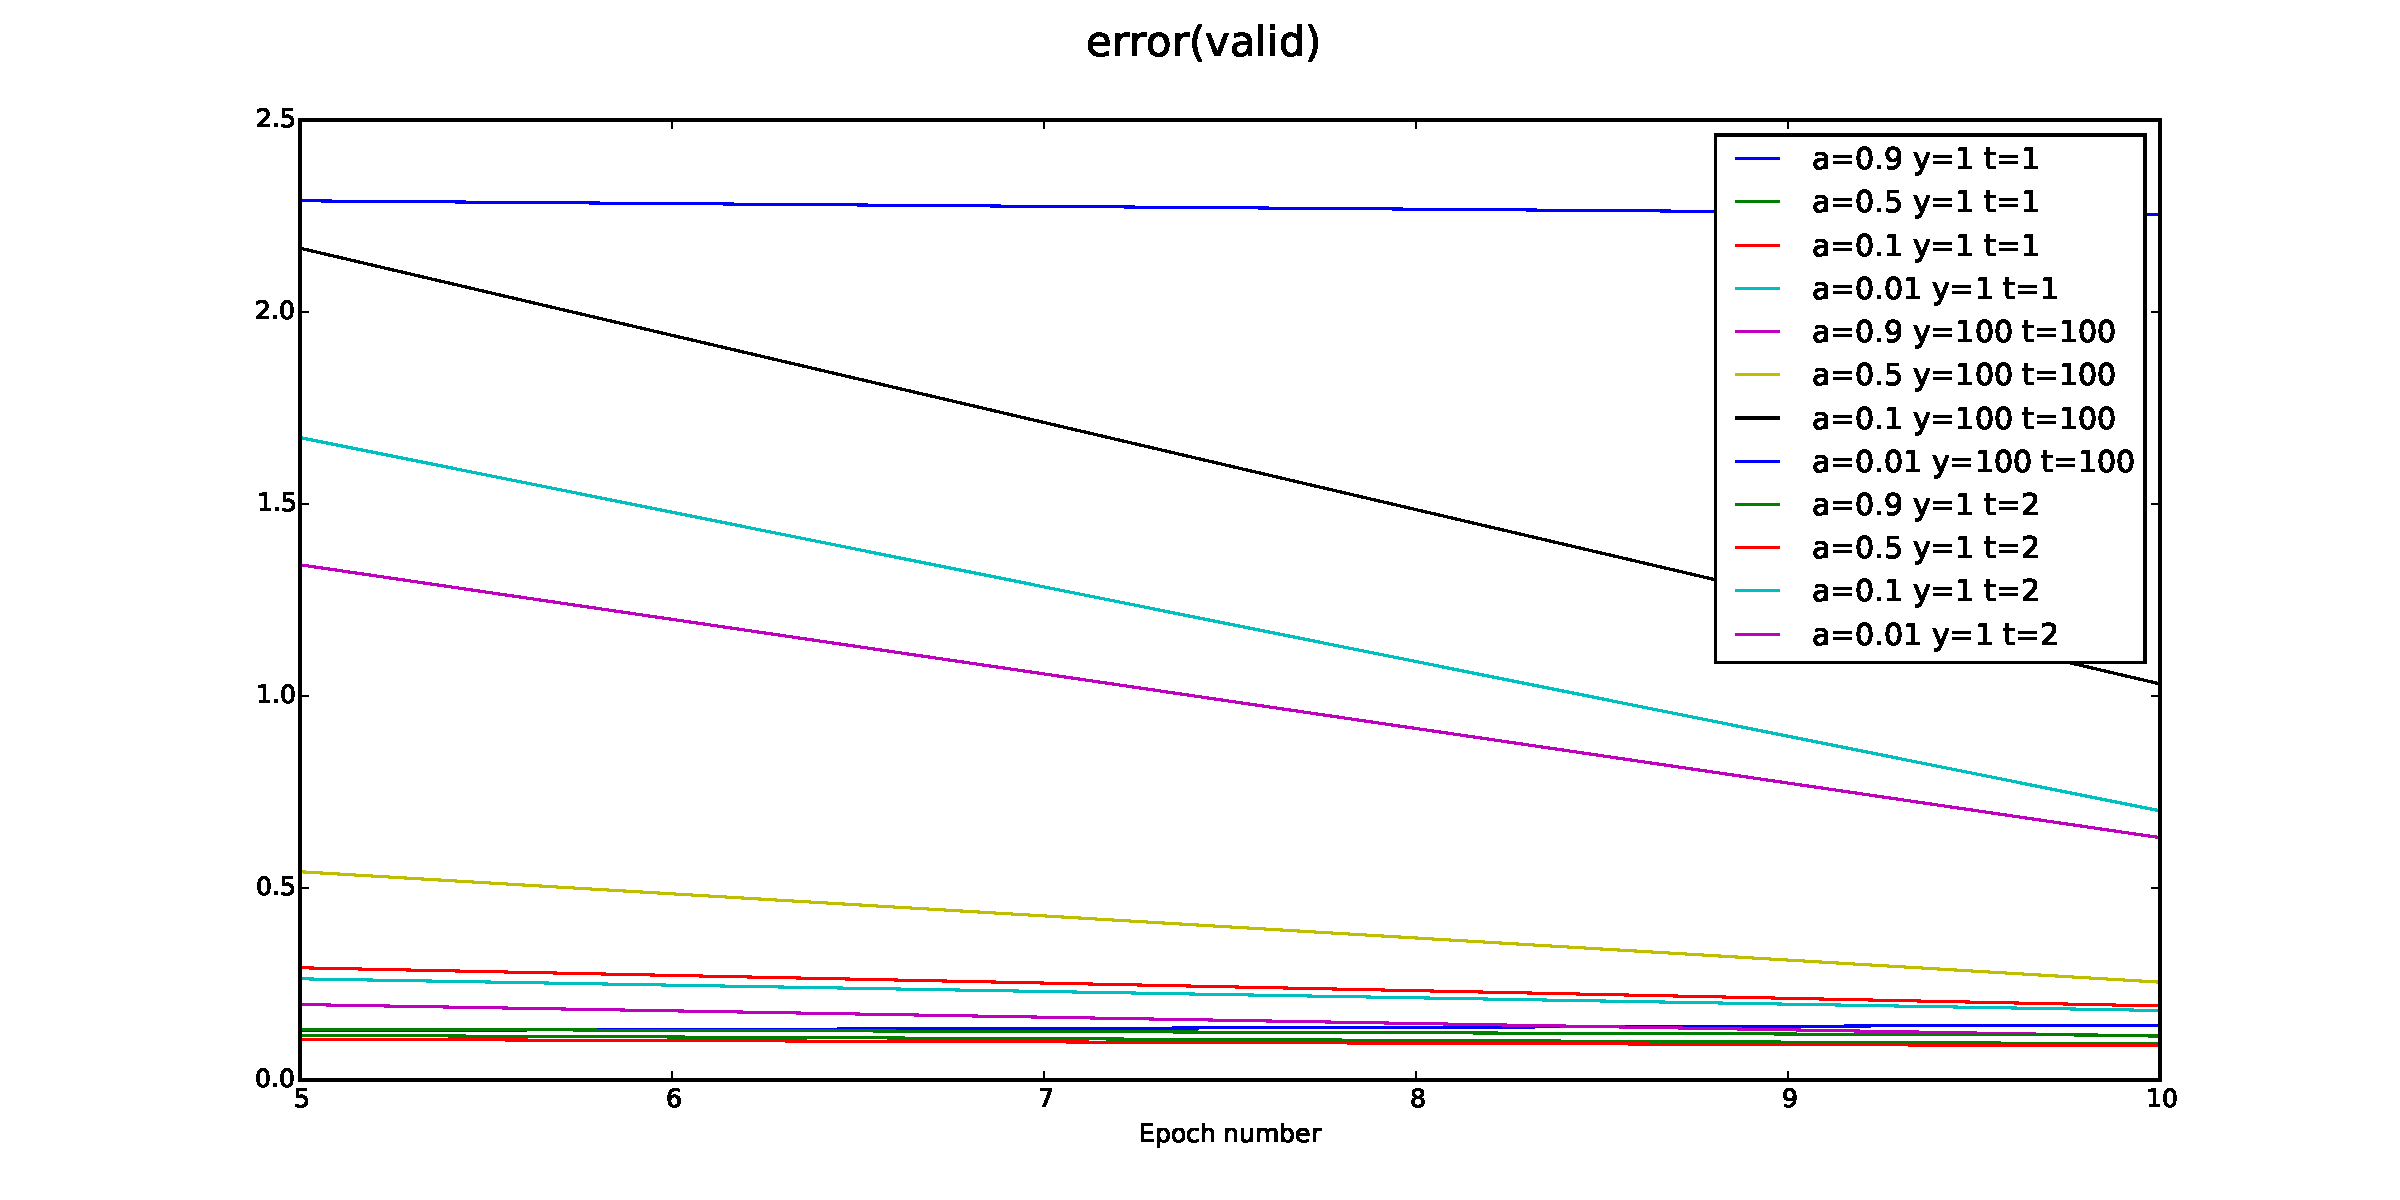
\includegraphics[width=9.1cm]{Task2/figures/Mome_var_error(valid).pdf}
\end{subfigure}%
\end{figure}
\begin{figure}[h]
\centering
\begin{subfigure}{.5\textwidth}
  \centering
  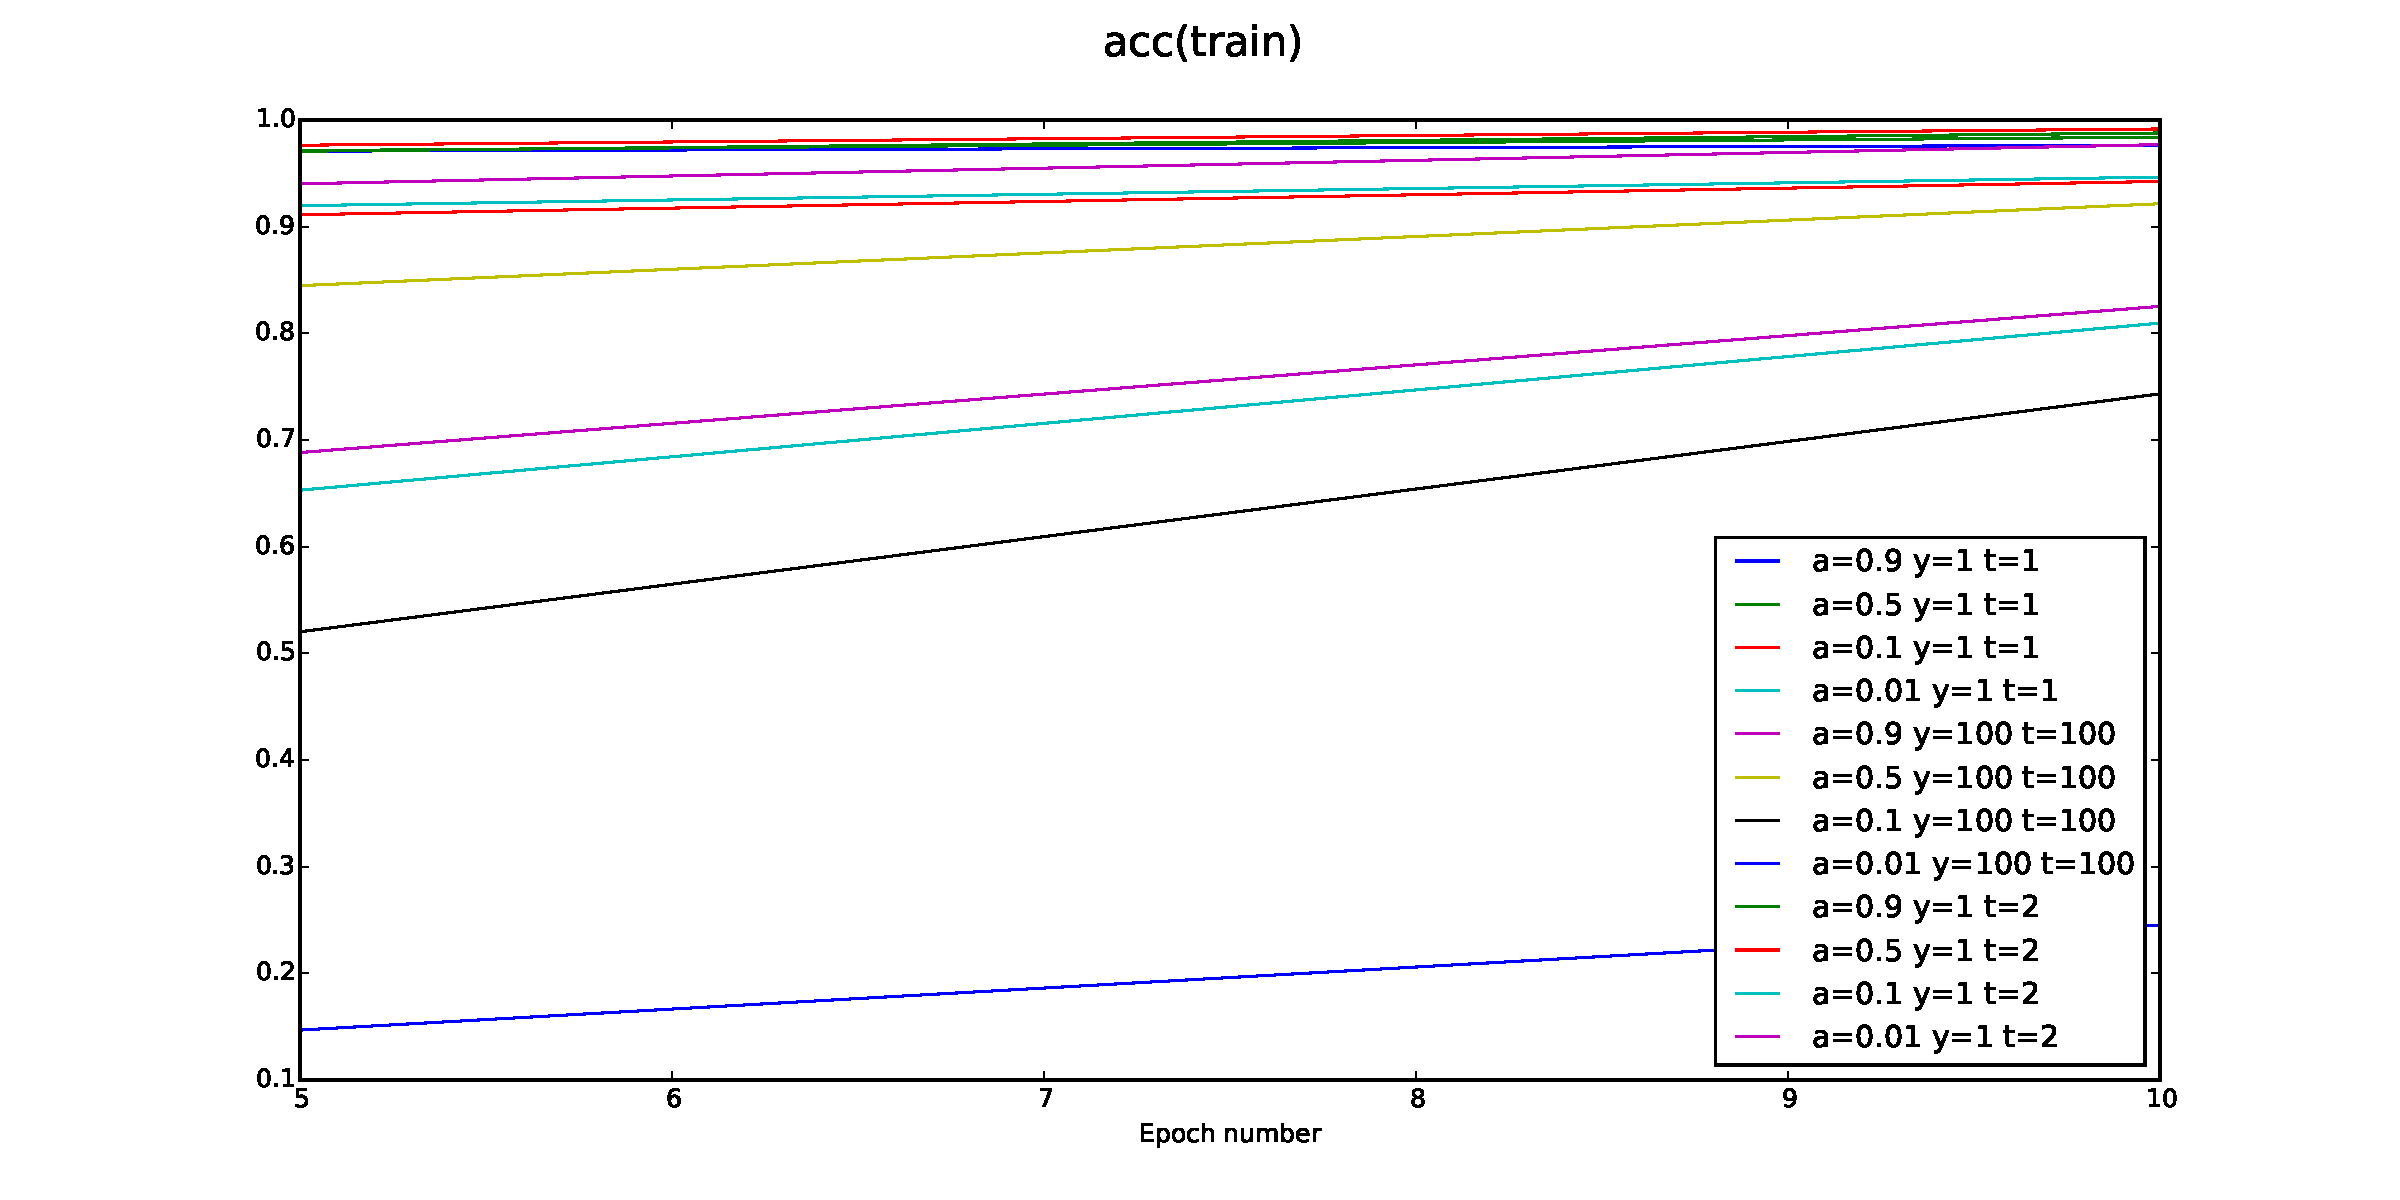
\includegraphics[width=9.1cm]{Task2/figures/Mome_var_acc(train).pdf}
\end{subfigure}%
\begin{subfigure}{.5\textwidth}
  \centering
  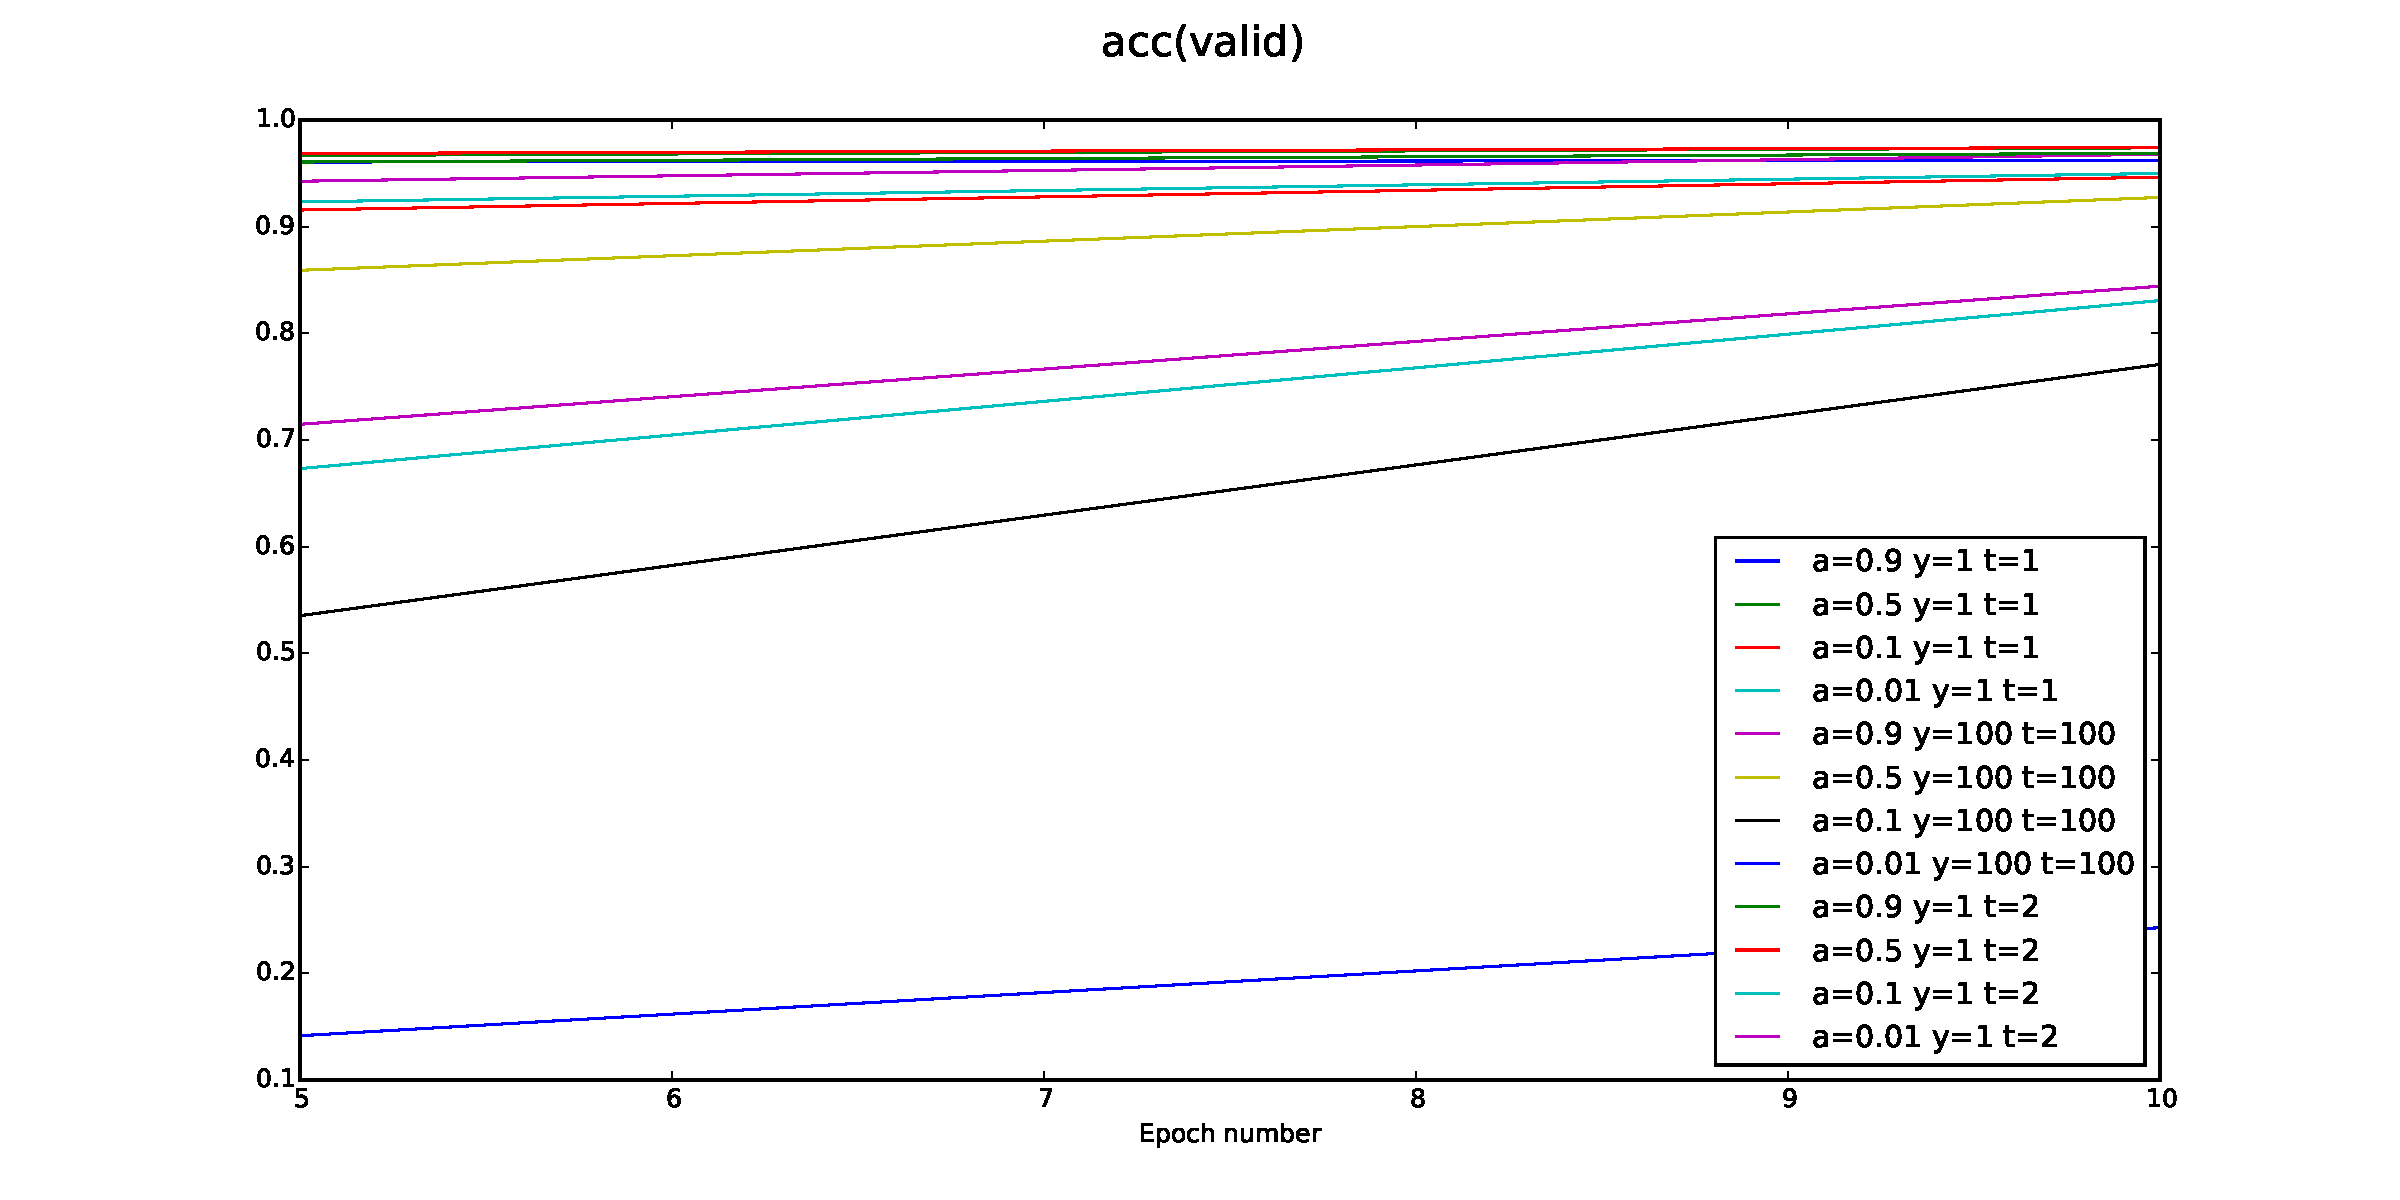
\includegraphics[width=9.1cm]{Task2/figures/Mome_var_acc(valid).pdf}
\end{subfigure}%
  \caption{Decaying momentum learning rule hyperparameter results.}
  \label{fig:mome_var}
  
\end{figure}

\begin{figure}[h]
\centering
\begin{subfigure}{.5\textwidth}
\centering
\begin{tabular}[h]{| c | c |}
\hline
Alhpa &  Accuracy(valid) \\
\hline
0.99 & 0.8342 \\
\hline
0.95 & 0.9781 \\
\hline
0.9 & 0.9788 \\
\hline
0.85 & 0.9784 \\
\hline
0.8 & 0.9779 \\
\hline
0.6 & 0.9788 \\
\hline
0.4 & 0.9784 \\
\hline
0.2 & 0.9791 \\
\hline
0.1 & 0.9797 \\
\hline
0.05 & 0.9797 \\
\hline
0.01 & 0.9799 \\
\hline
0.001 & 0.9799 \\
\hline
\end{tabular}
\end{subfigure}%
\begin{subfigure}{.5\textwidth}

\centering
\begin{tabular}[h]{| c | c | c | c |}
\hline
Alhpa & Gamma & Tau &  Accuracy(valid) \\
\hline
0.9 & 1 & 1 & 0.9622 \\
\hline
0.5 & 1 & 1 & 0.9739 \\
\hline
0.1 & 1 & 1 & 0.9464 \\
\hline
0.01 & 1 & 1 & 0.8307 \\
\hline
0.9 & 100 & 100 & 0.9679 \\
\hline
0.5 & 100 & 100 & 0.9274 \\
\hline
0.1 & 100 & 100 & 0.7709 \\
\hline
0.01 & 100 & 100 & 0.2428 \\
\hline
0.9 & 1 & 2 & 0.9688 \\
\hline
0.5 & 1 & 2 & 0.9743 \\
\hline
0.1 & 1 & 2 & 0.9499 \\
\hline
0.01 & 1 & 2 & 0.8442 \\
\hline
\end{tabular}
\end{subfigure}%

  \caption{Comparison of momentum hyperparameters on accuracy/}
  \label{fig:task2_table}
\end{figure}

  Figure \ref{fig:task2_table} compares the time varying momentum to a constant learning schedule. It does not show a significant improvement on this dataset.




\section*{Task 3 - Adaptive learning rules }
The last section explores adaptive learning rates, namely AdaGrad and RMSProp. Both of these rules apply updates to each weight individually. AdaGrad normalizes each weight parameter, meaning that weights with larger gradient magnitudes will have smaller weight updates and small gradients will result in larger updates. 
\[ S_i(t) =S_i(t-1) + D_i(t)^2\] 
\[ cw_i(t) = -n/(\surd(S_i(t)+e)*D_i(t) \] 
In the equation above D is the gradient and e is a small constant (1e-8) to prevent division by 0. 




\begin{figure}[h]
\centering
\begin{subfigure}{.5\textwidth}
  \centering
  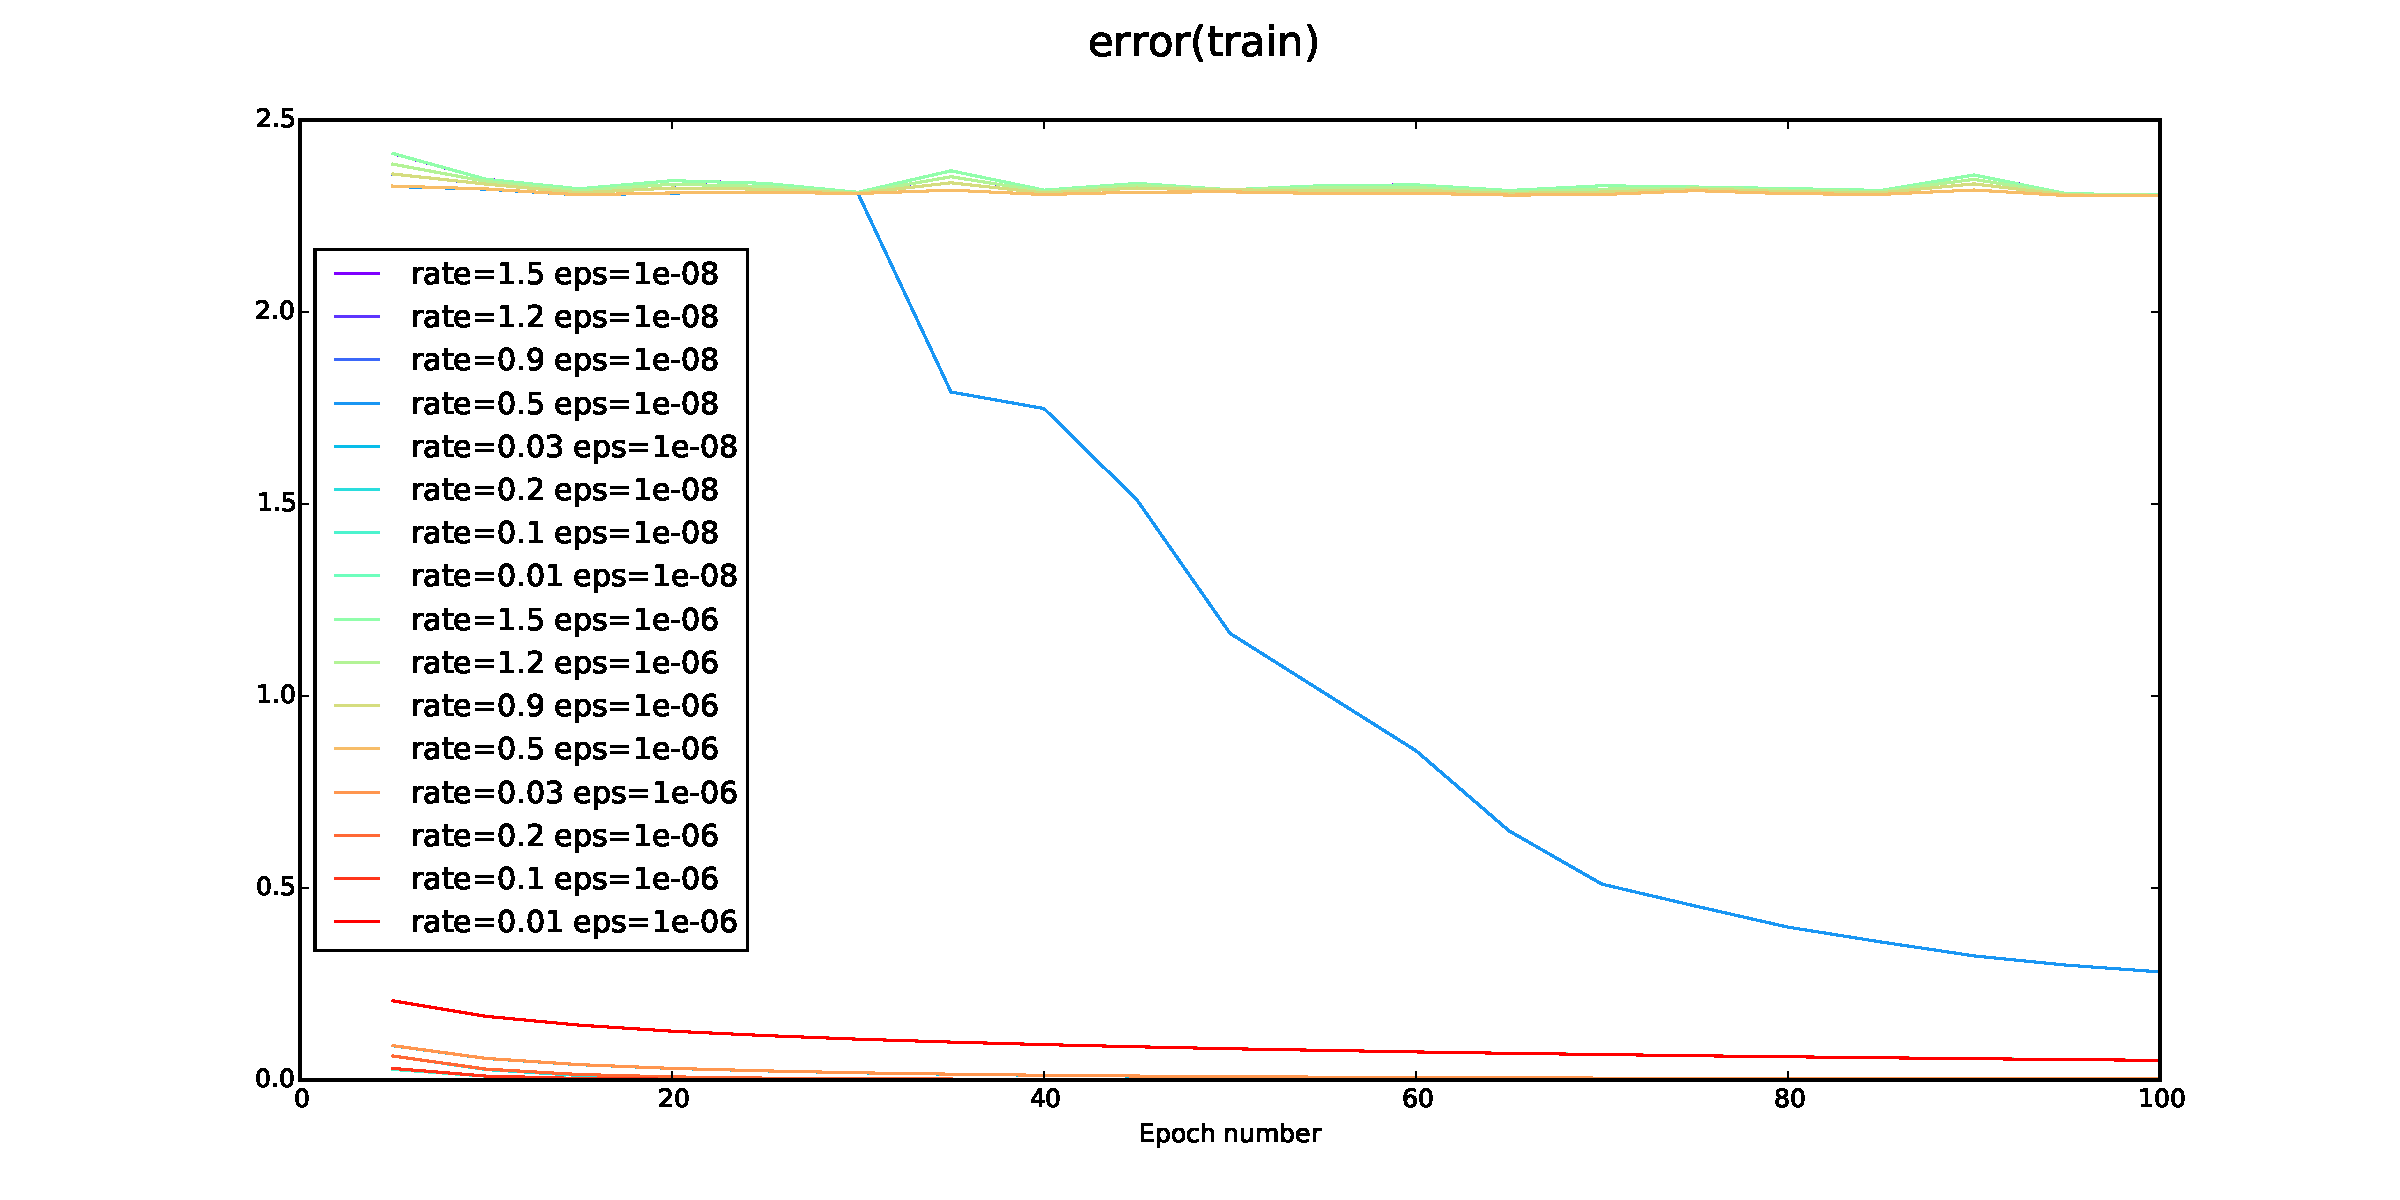
\includegraphics[width=9.1cm]{Task3/figures/Ada_error(train).pdf}
\end{subfigure}%
\begin{subfigure}{.5\textwidth}
  \centering
  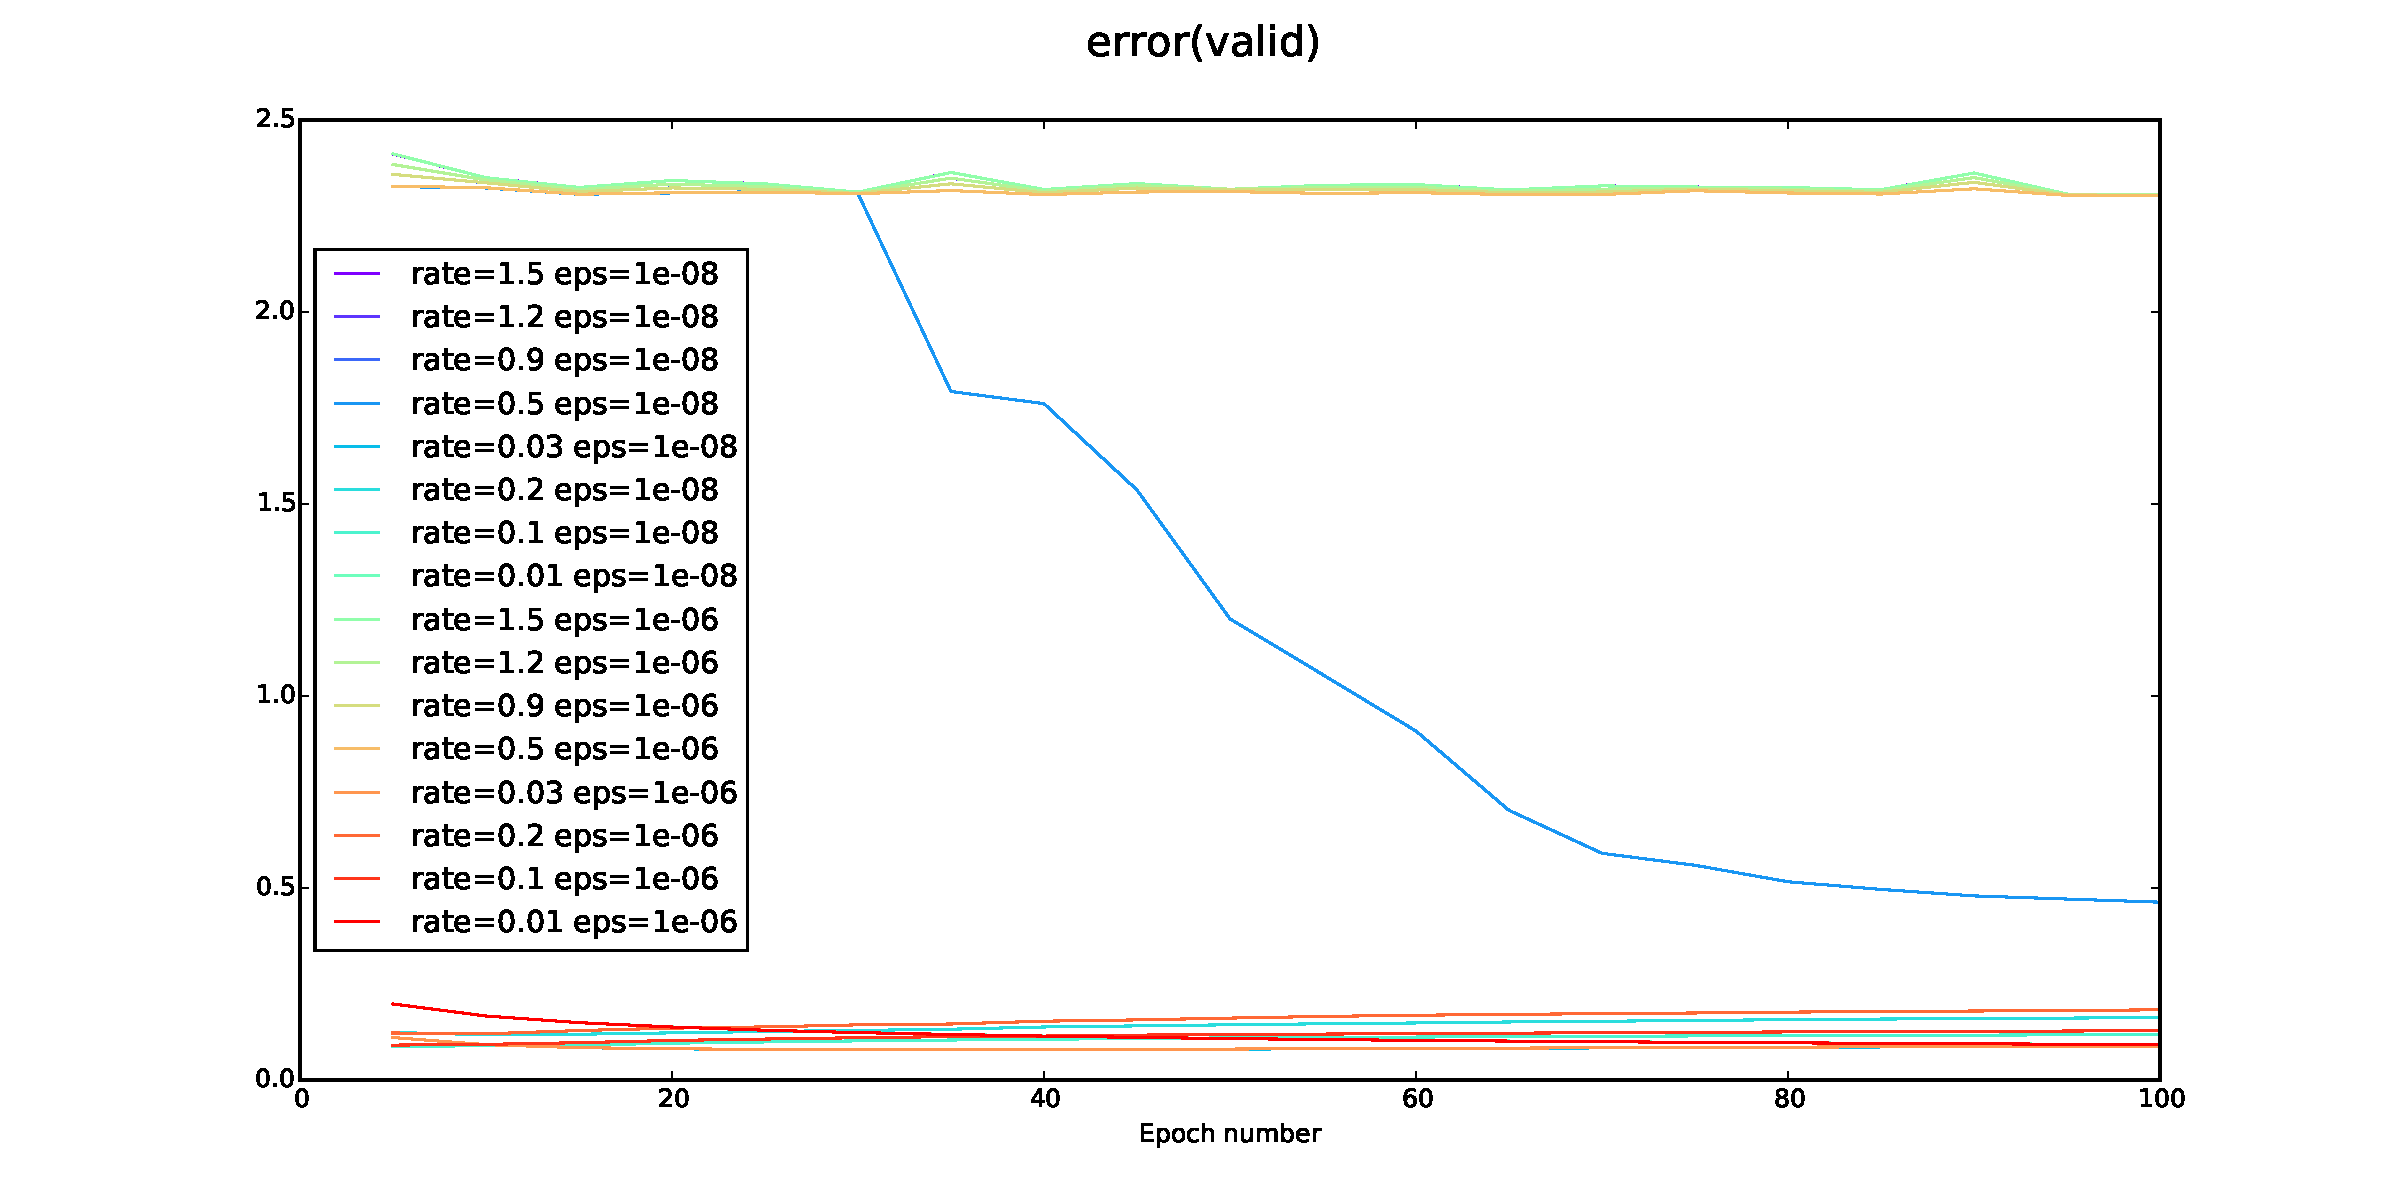
\includegraphics[width=9.1cm]{Task3/figures/Ada_error(valid).pdf}
\end{subfigure}%
\end{figure}
\begin{figure}[h]
\centering
\begin{subfigure}{.5\textwidth}
  \centering
  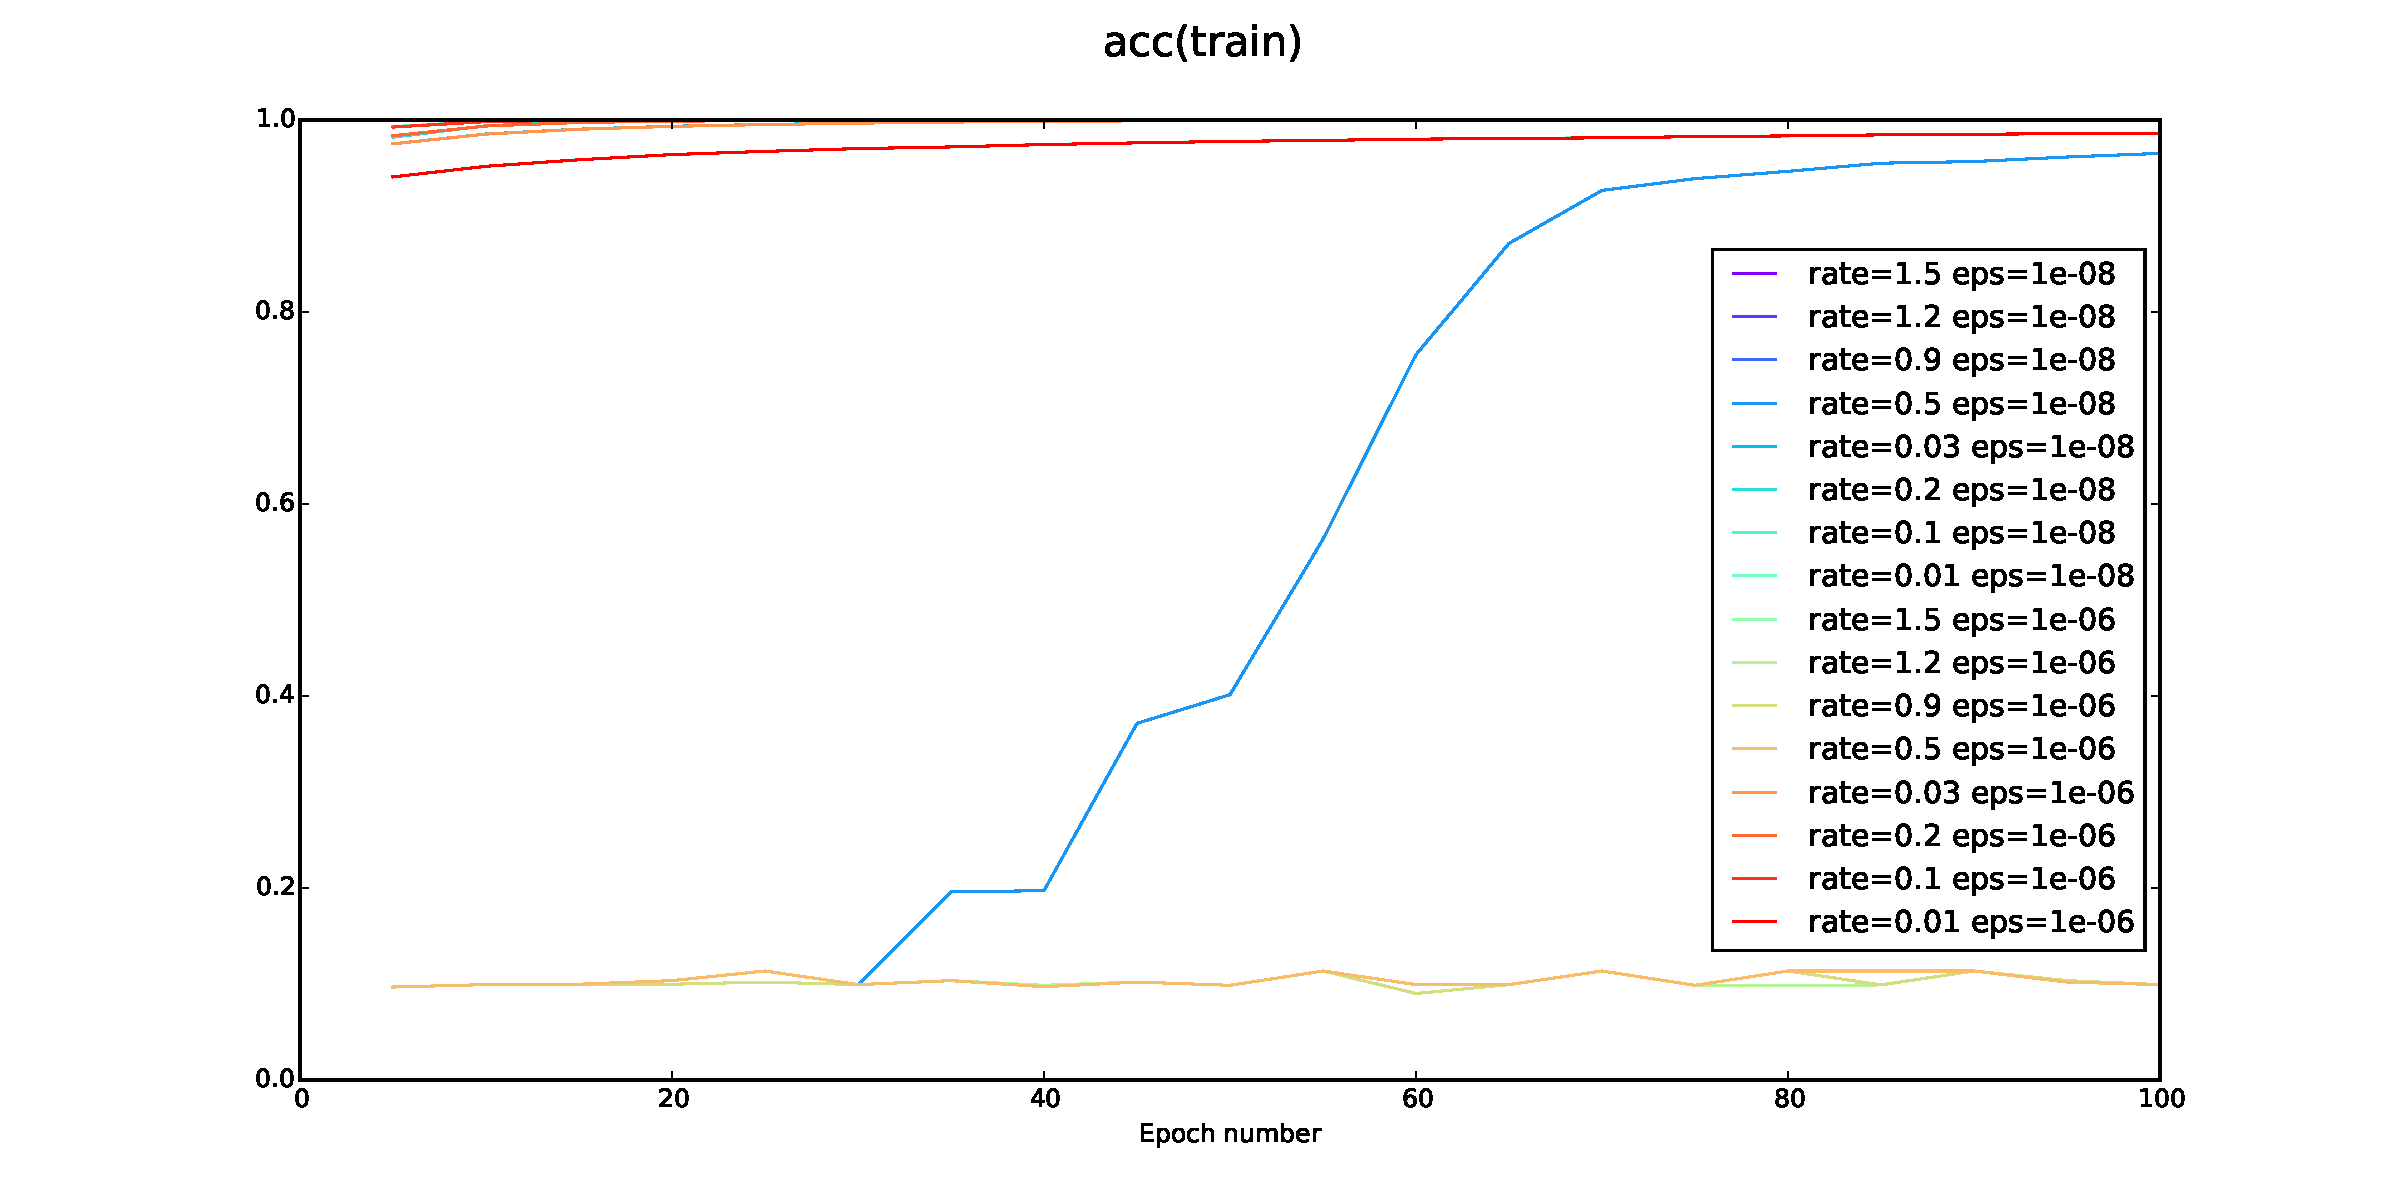
\includegraphics[width=9.1cm]{Task3/figures/Ada_acc(train).pdf}
\end{subfigure}%
\begin{subfigure}{.5\textwidth}
  \centering
  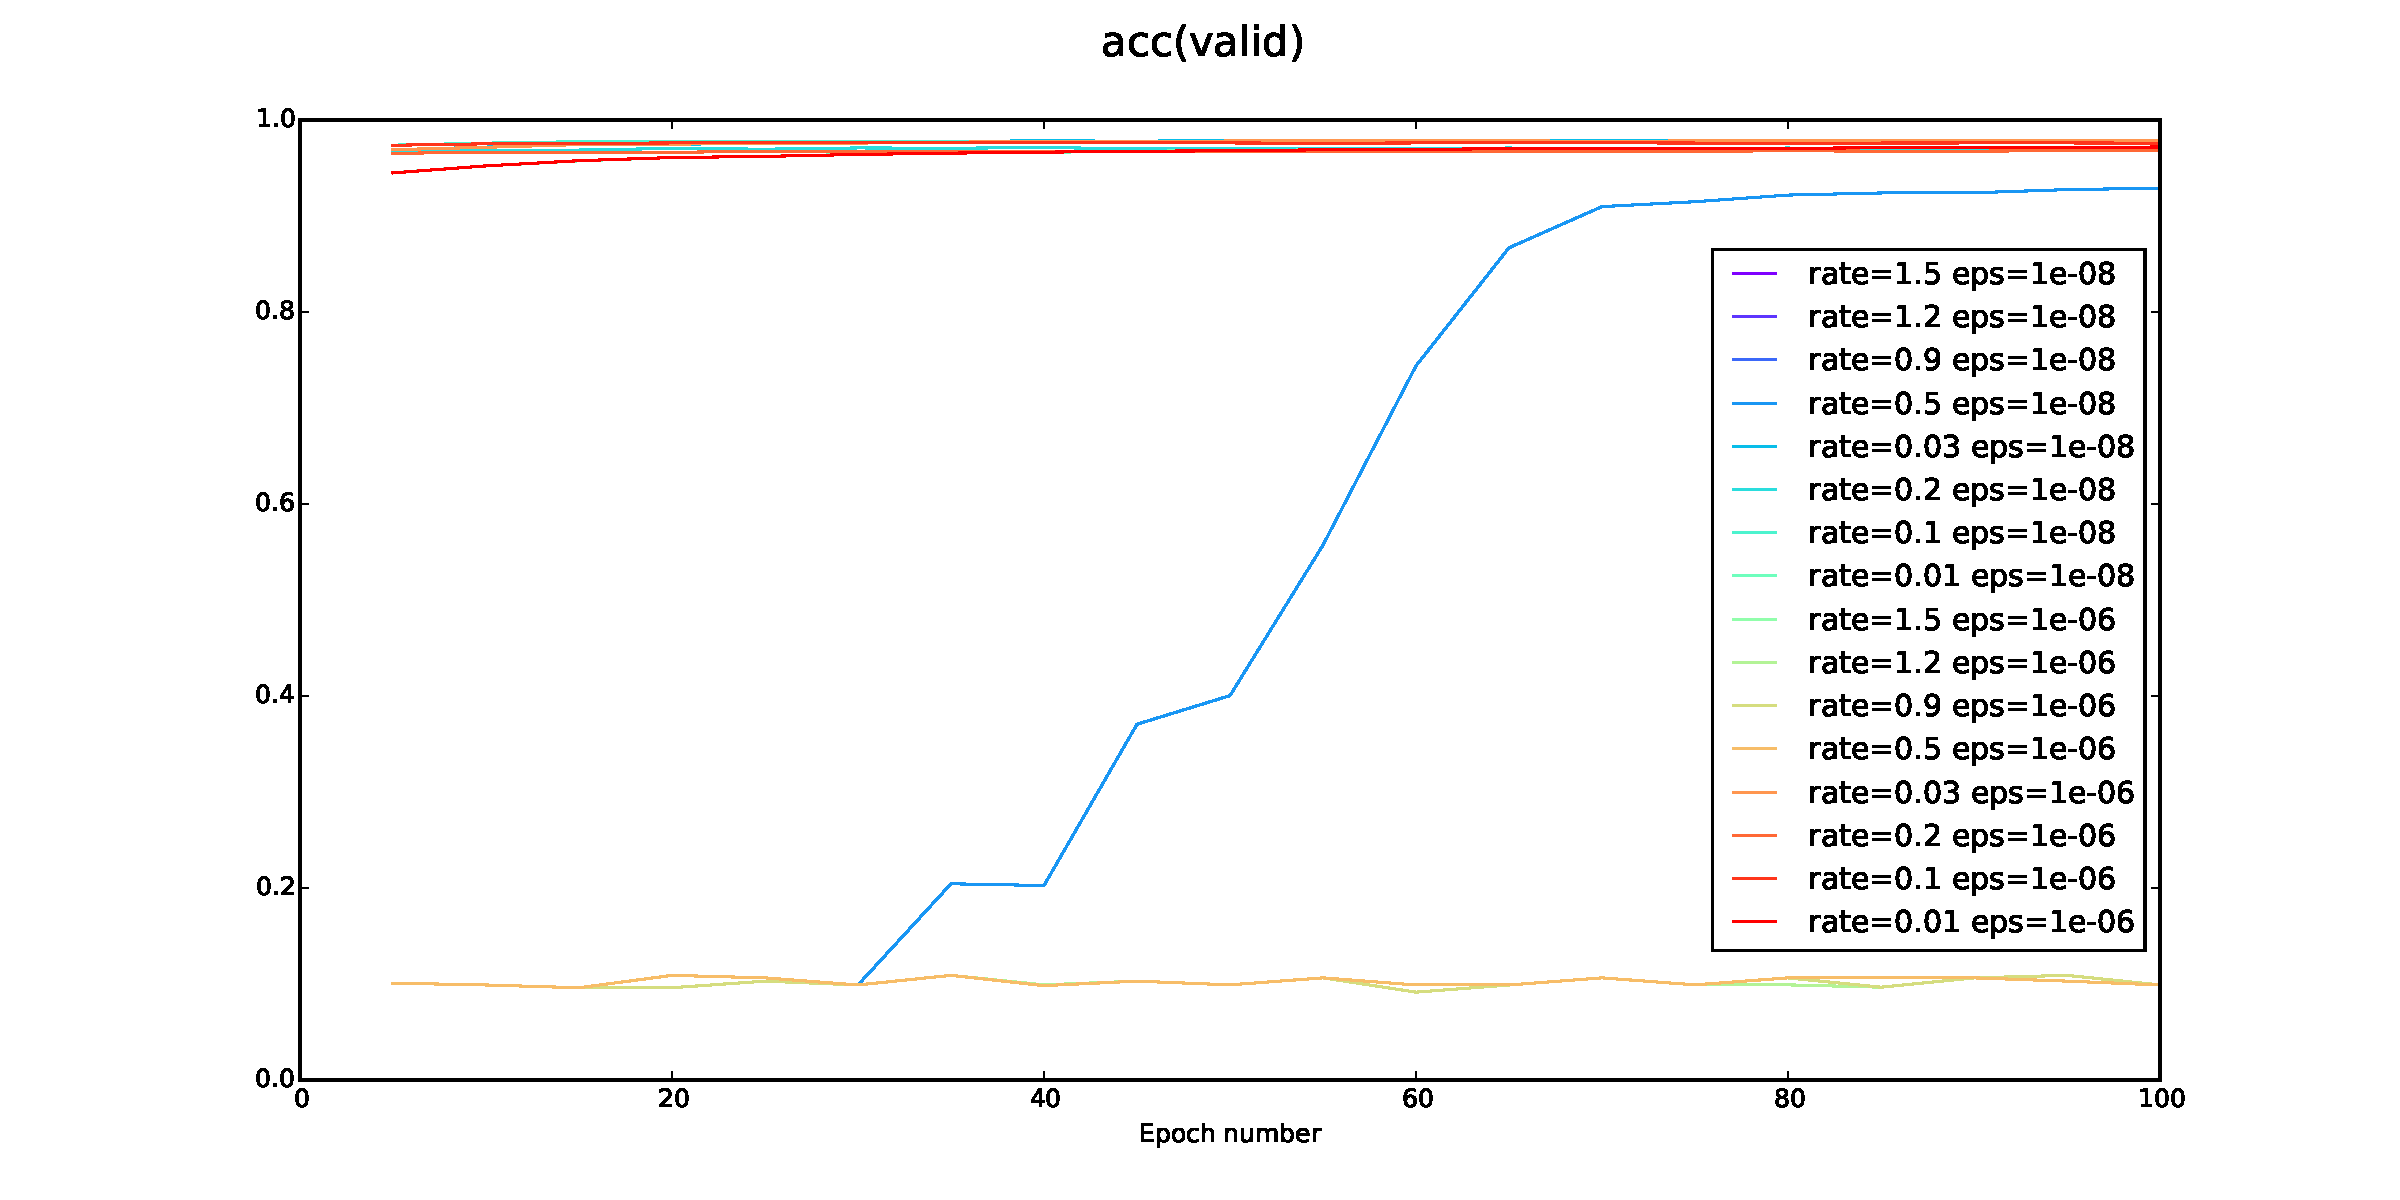
\includegraphics[width=9.1cm]{Task3/figures/Ada_acc(valid).pdf}
\end{subfigure}%
  \caption{AdaGrad learning rule hyperparameter results.}
  \label{fig:Ada}
\end{figure}

AdaGrad's performance is displayed in Figure \ref{fig:Ada}. The constant e should stay very small and the depended parameter is the learning rate showing similar results to constant learning rate. Both perform their best at learning rate 0.03. AdaGrad is more computationally intensive and learns quicker in terms of convergence but does not display enough of a boost to argue it's case over for example the exponential learning rate decay with gradient descent.

\begin{figure}[h]
\centering
\begin{subfigure}{.5\textwidth}
  \centering
  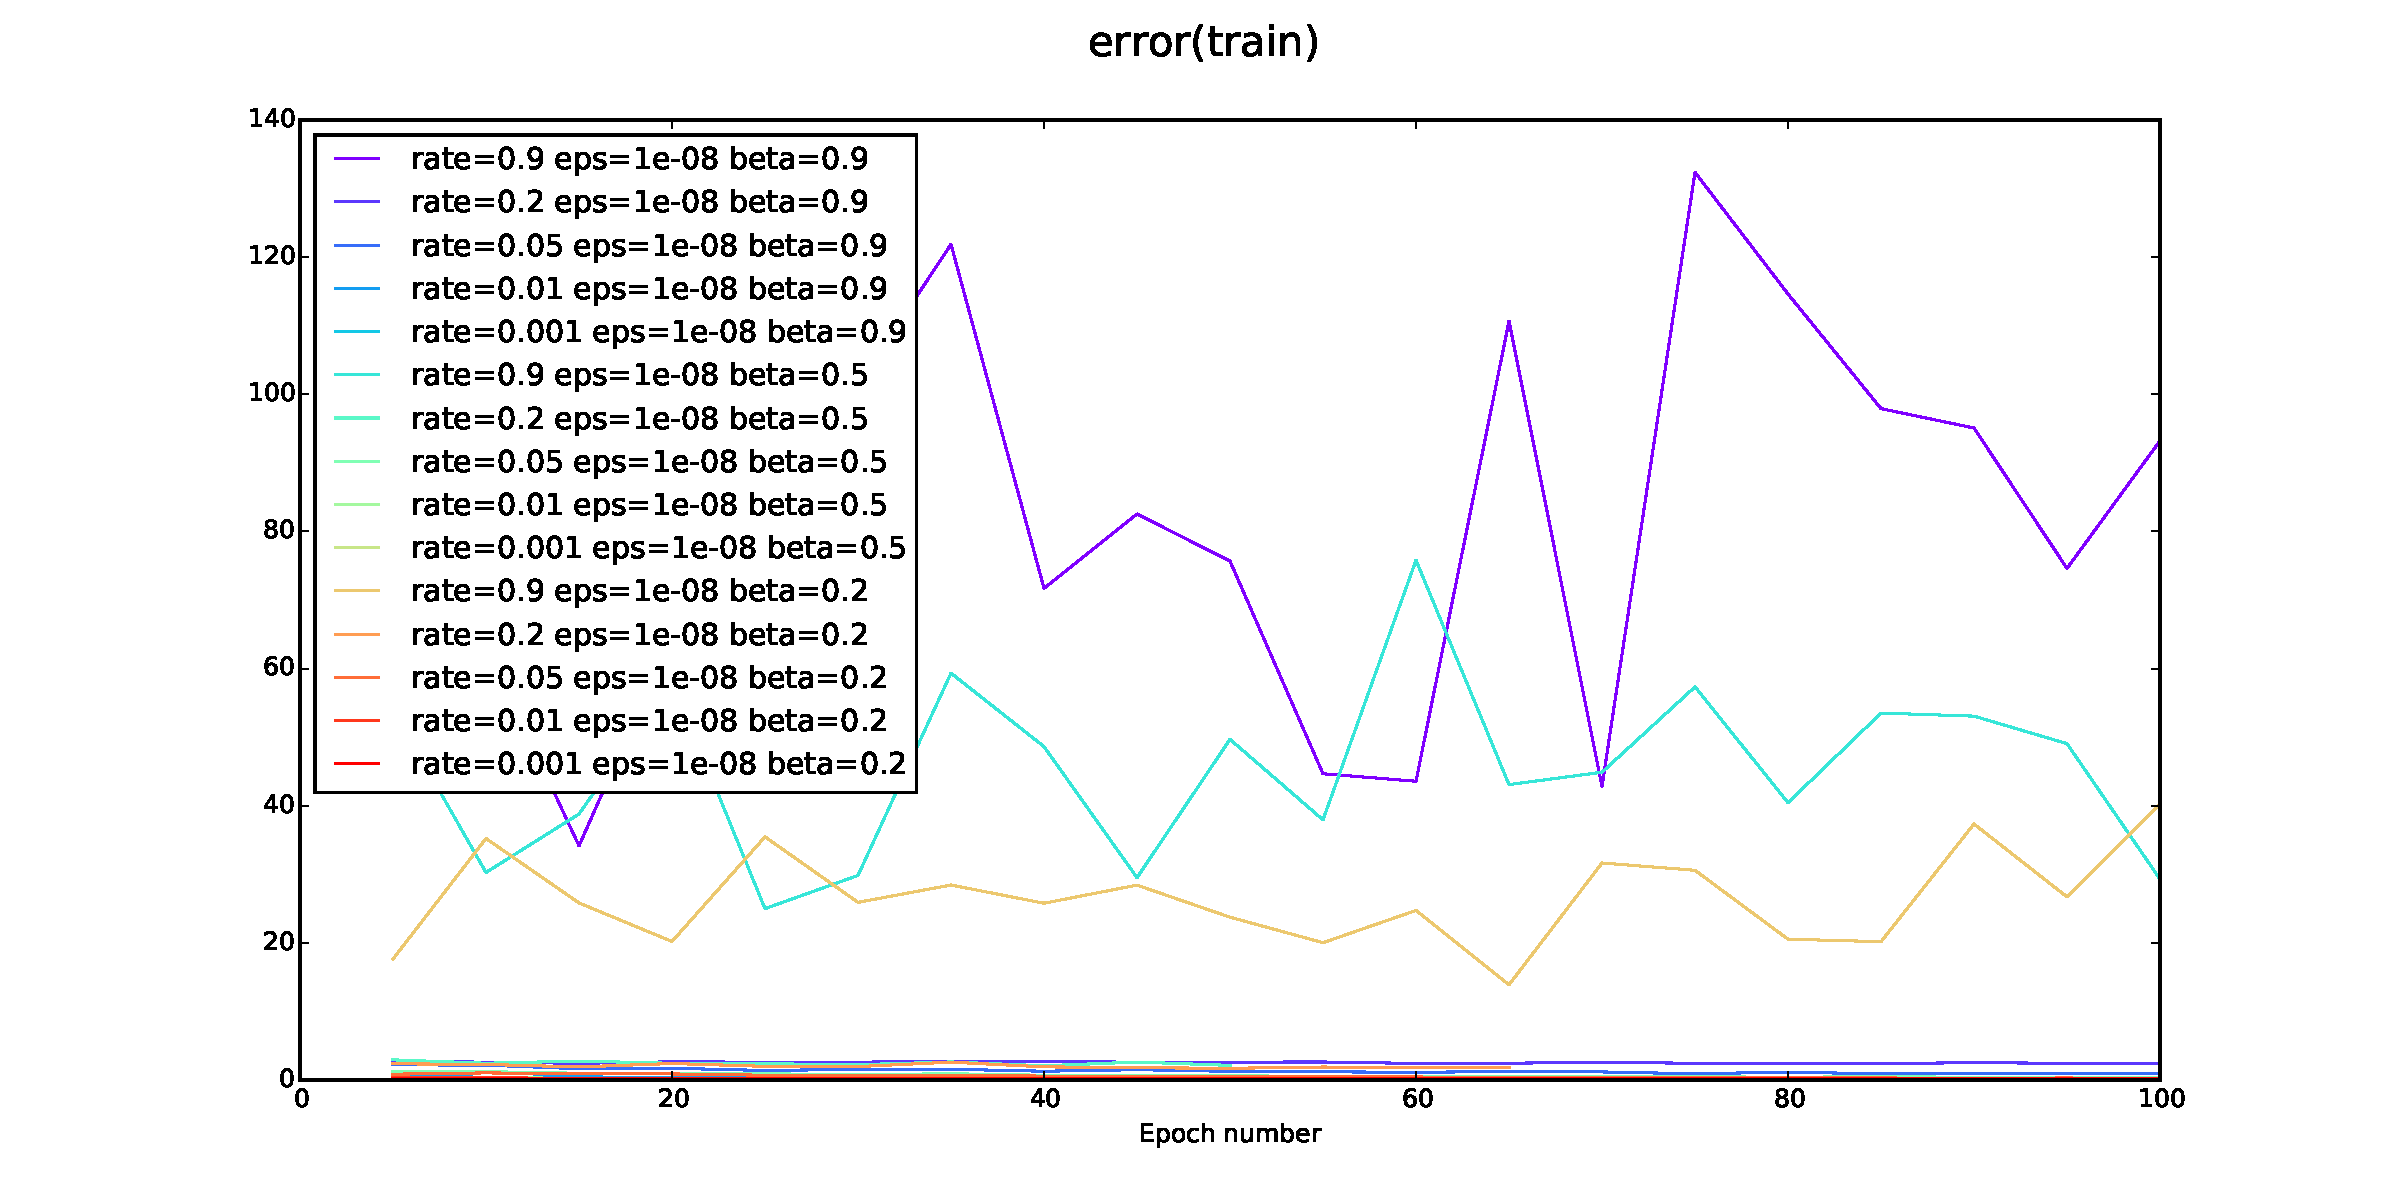
\includegraphics[width=9.1cm]{Task3/figures/Rms_error(train).pdf}
\end{subfigure}%
\begin{subfigure}{.5\textwidth}
  \centering
  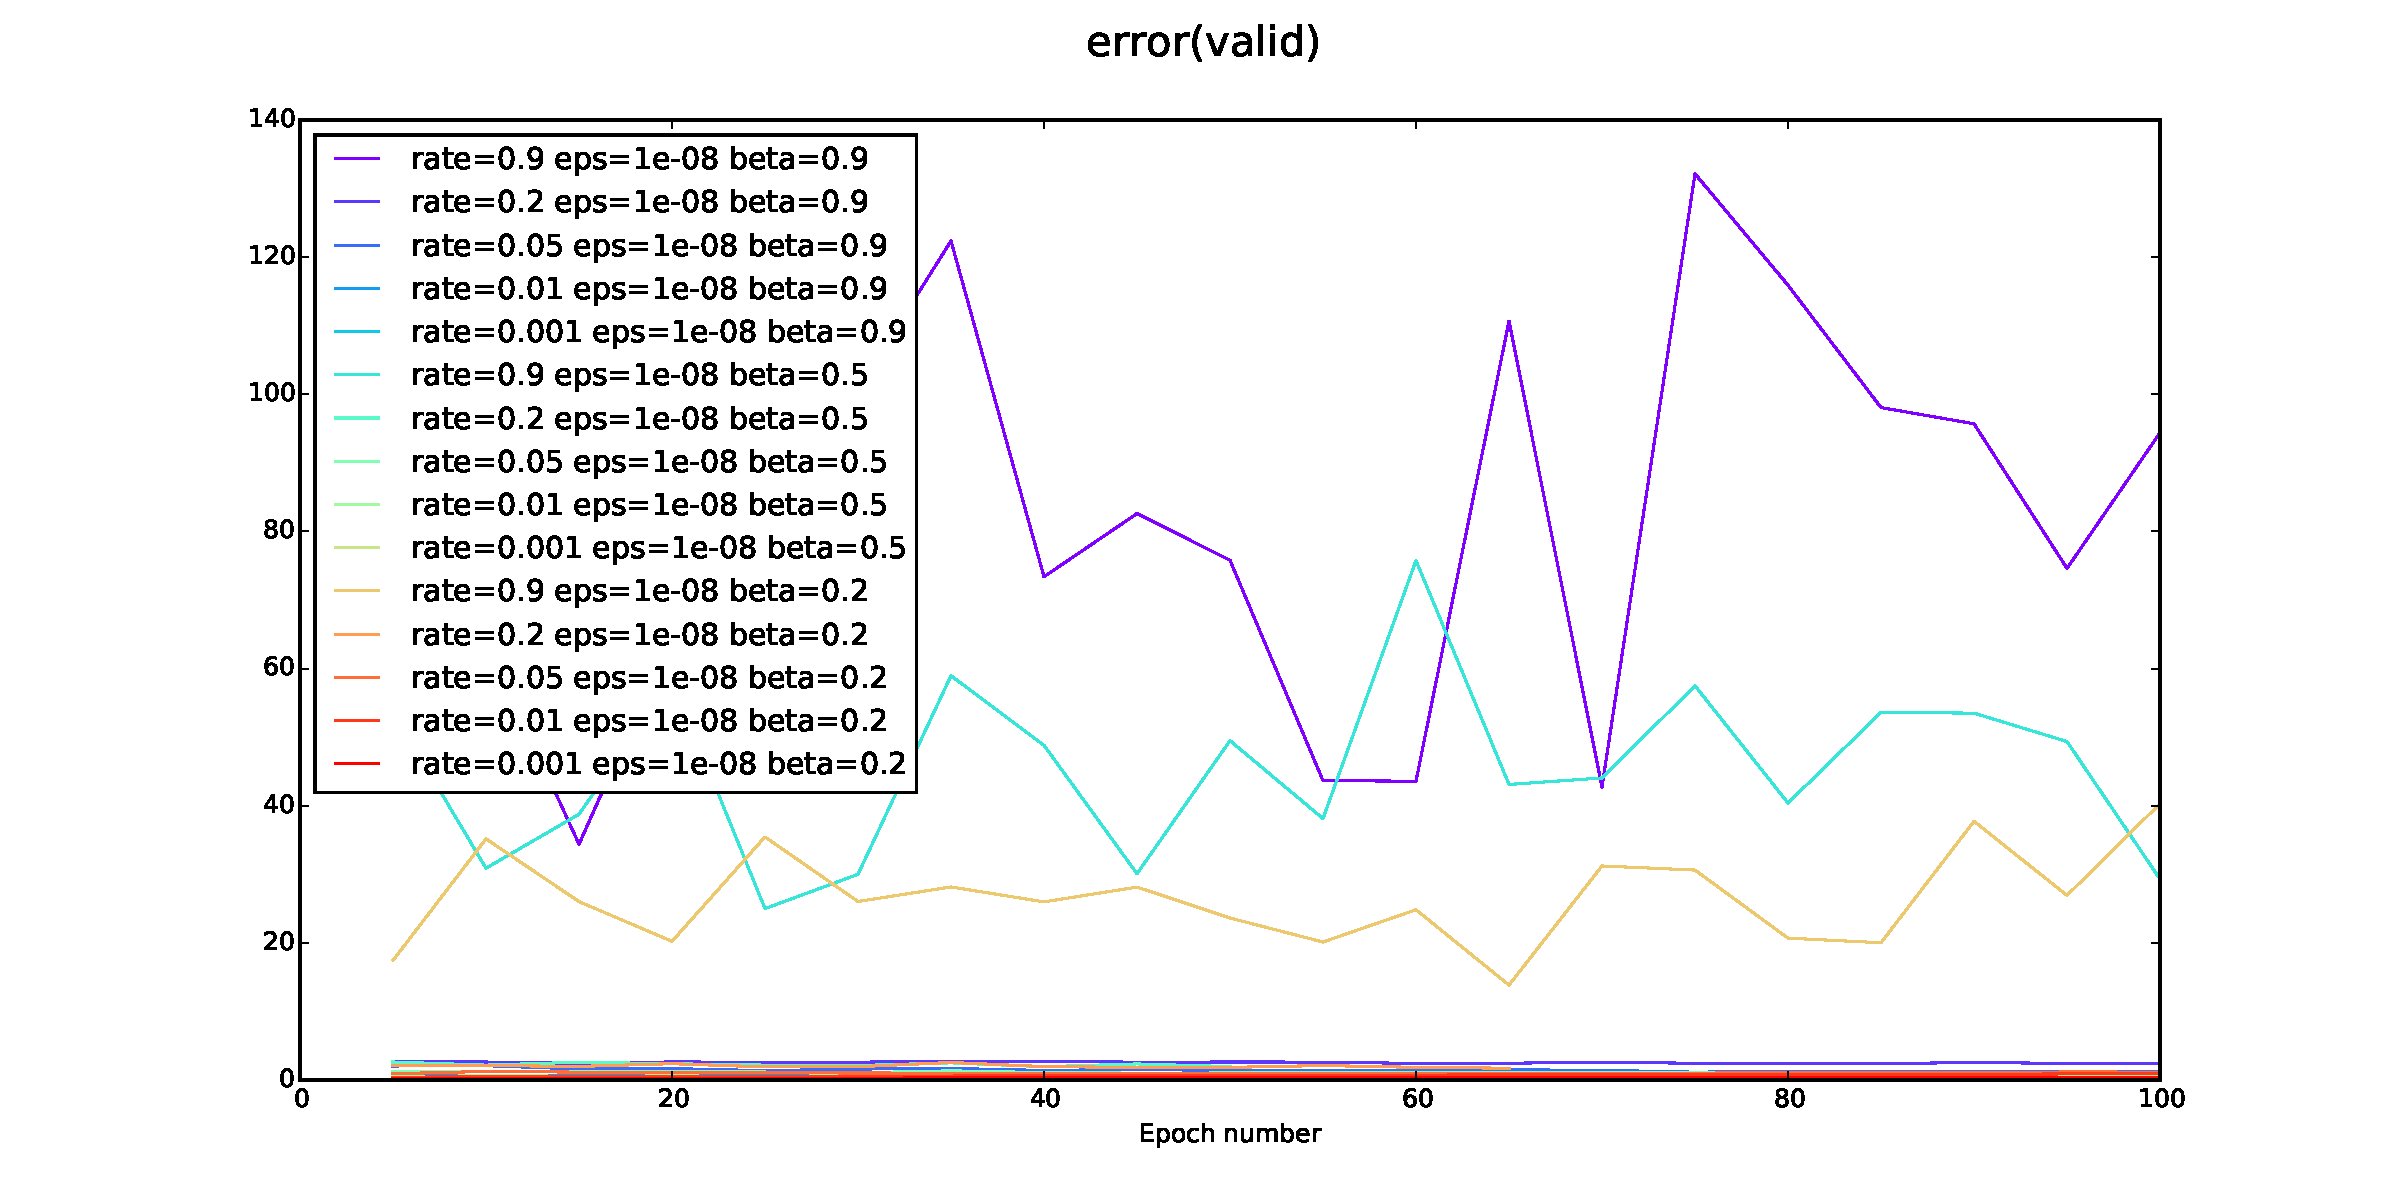
\includegraphics[width=9.1cm]{Task3/figures/Rms_error(valid).pdf}
\end{subfigure}%
\end{figure}
\begin{figure}[h]
\centering
\begin{subfigure}{.5\textwidth}
  \centering
  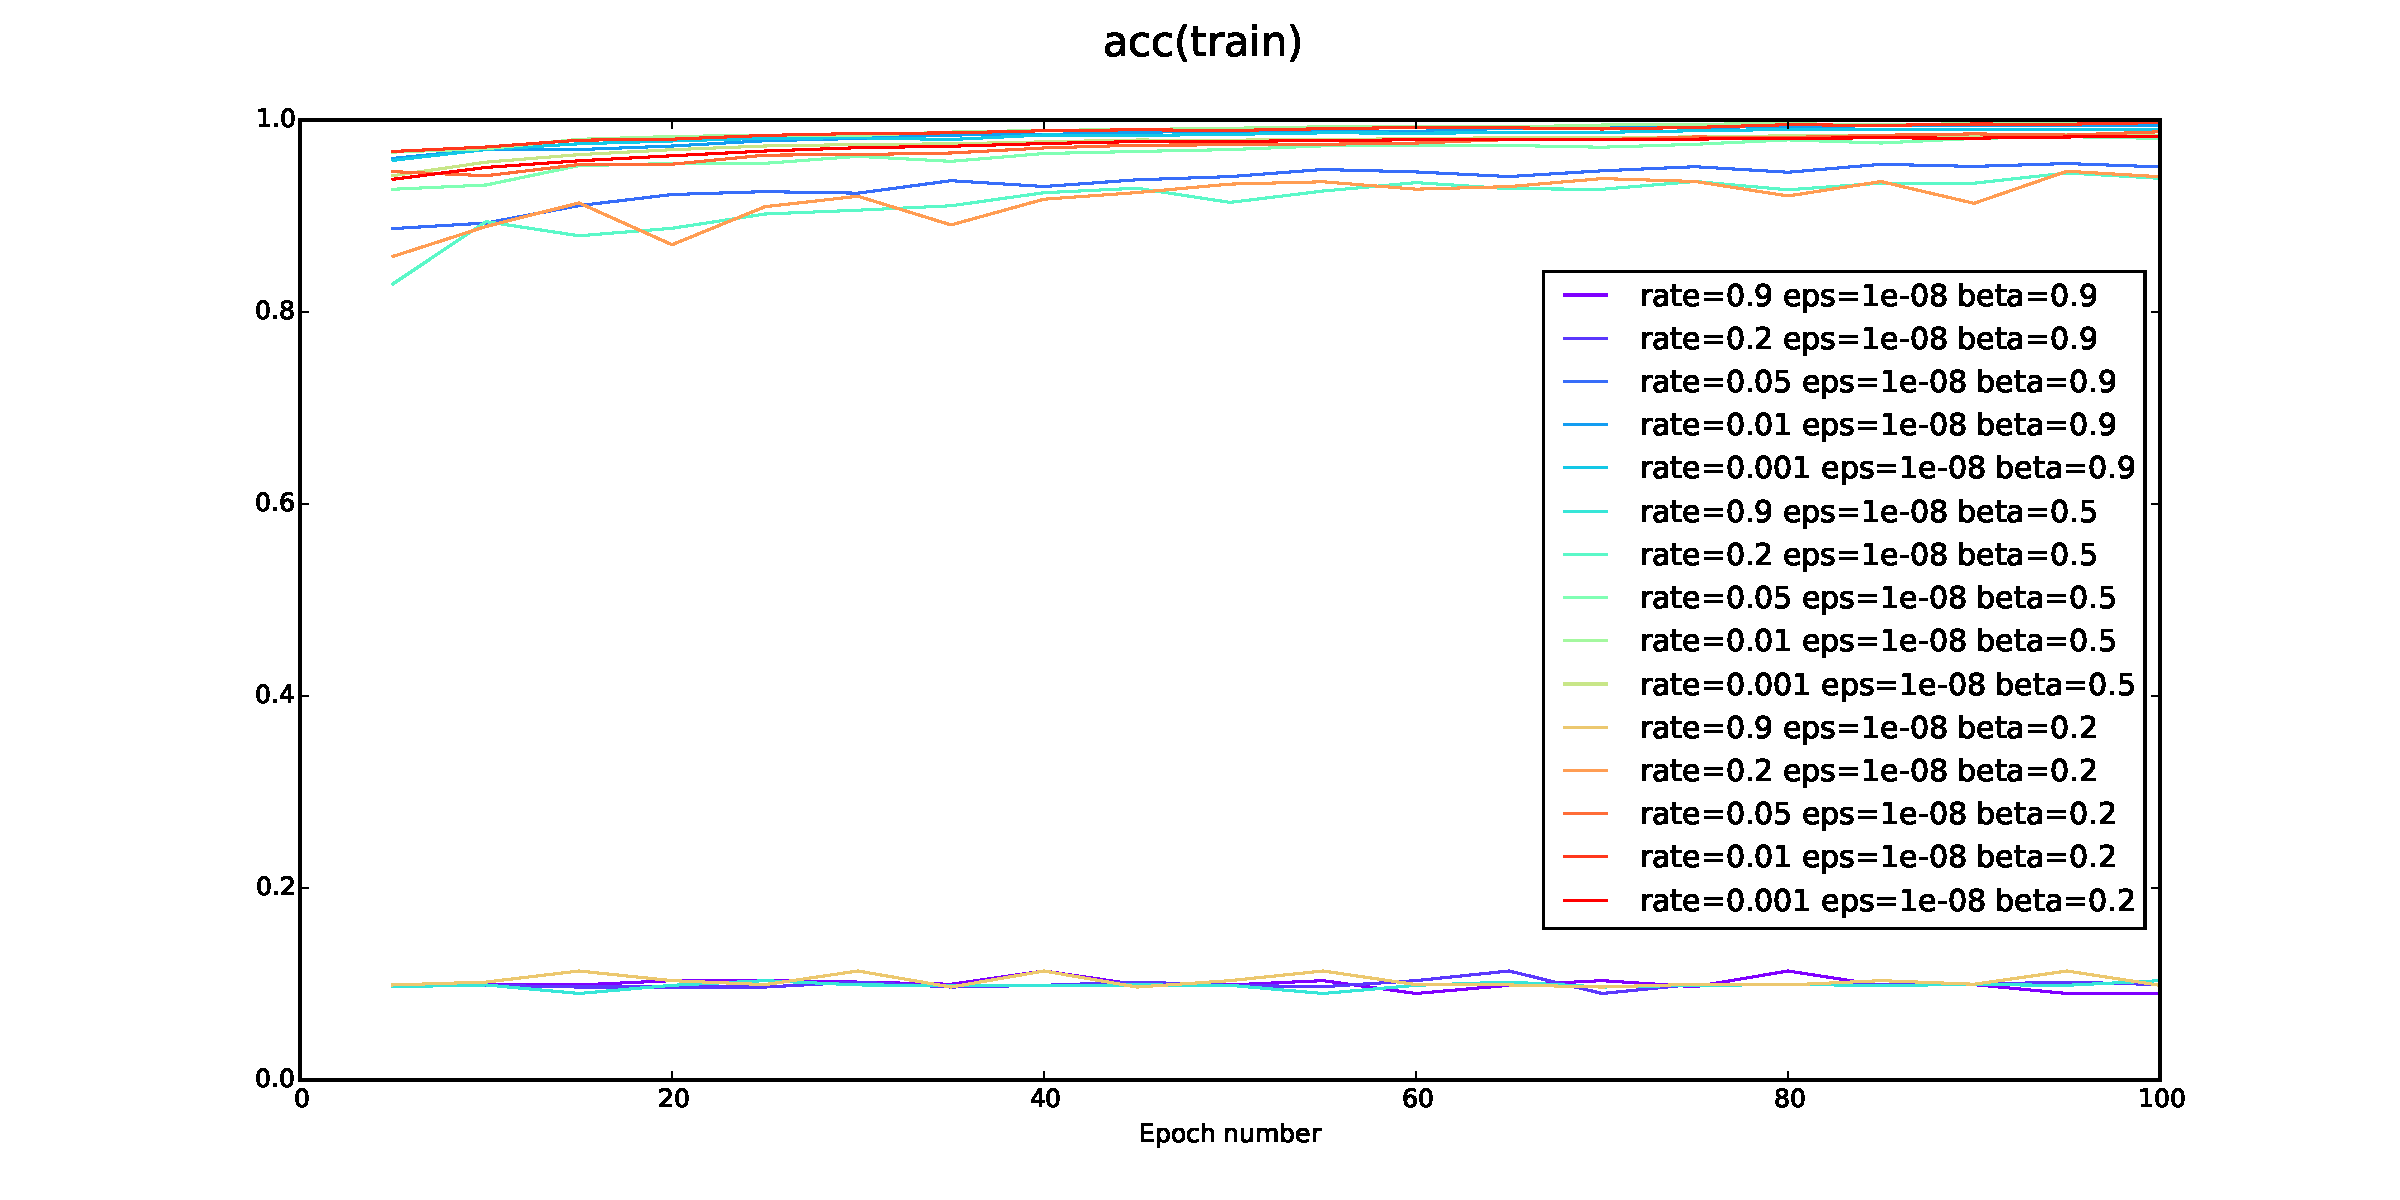
\includegraphics[width=9.1cm]{Task3/figures/Rms_acc(train).pdf}
\end{subfigure}%
\begin{subfigure}{.5\textwidth}
  \centering
  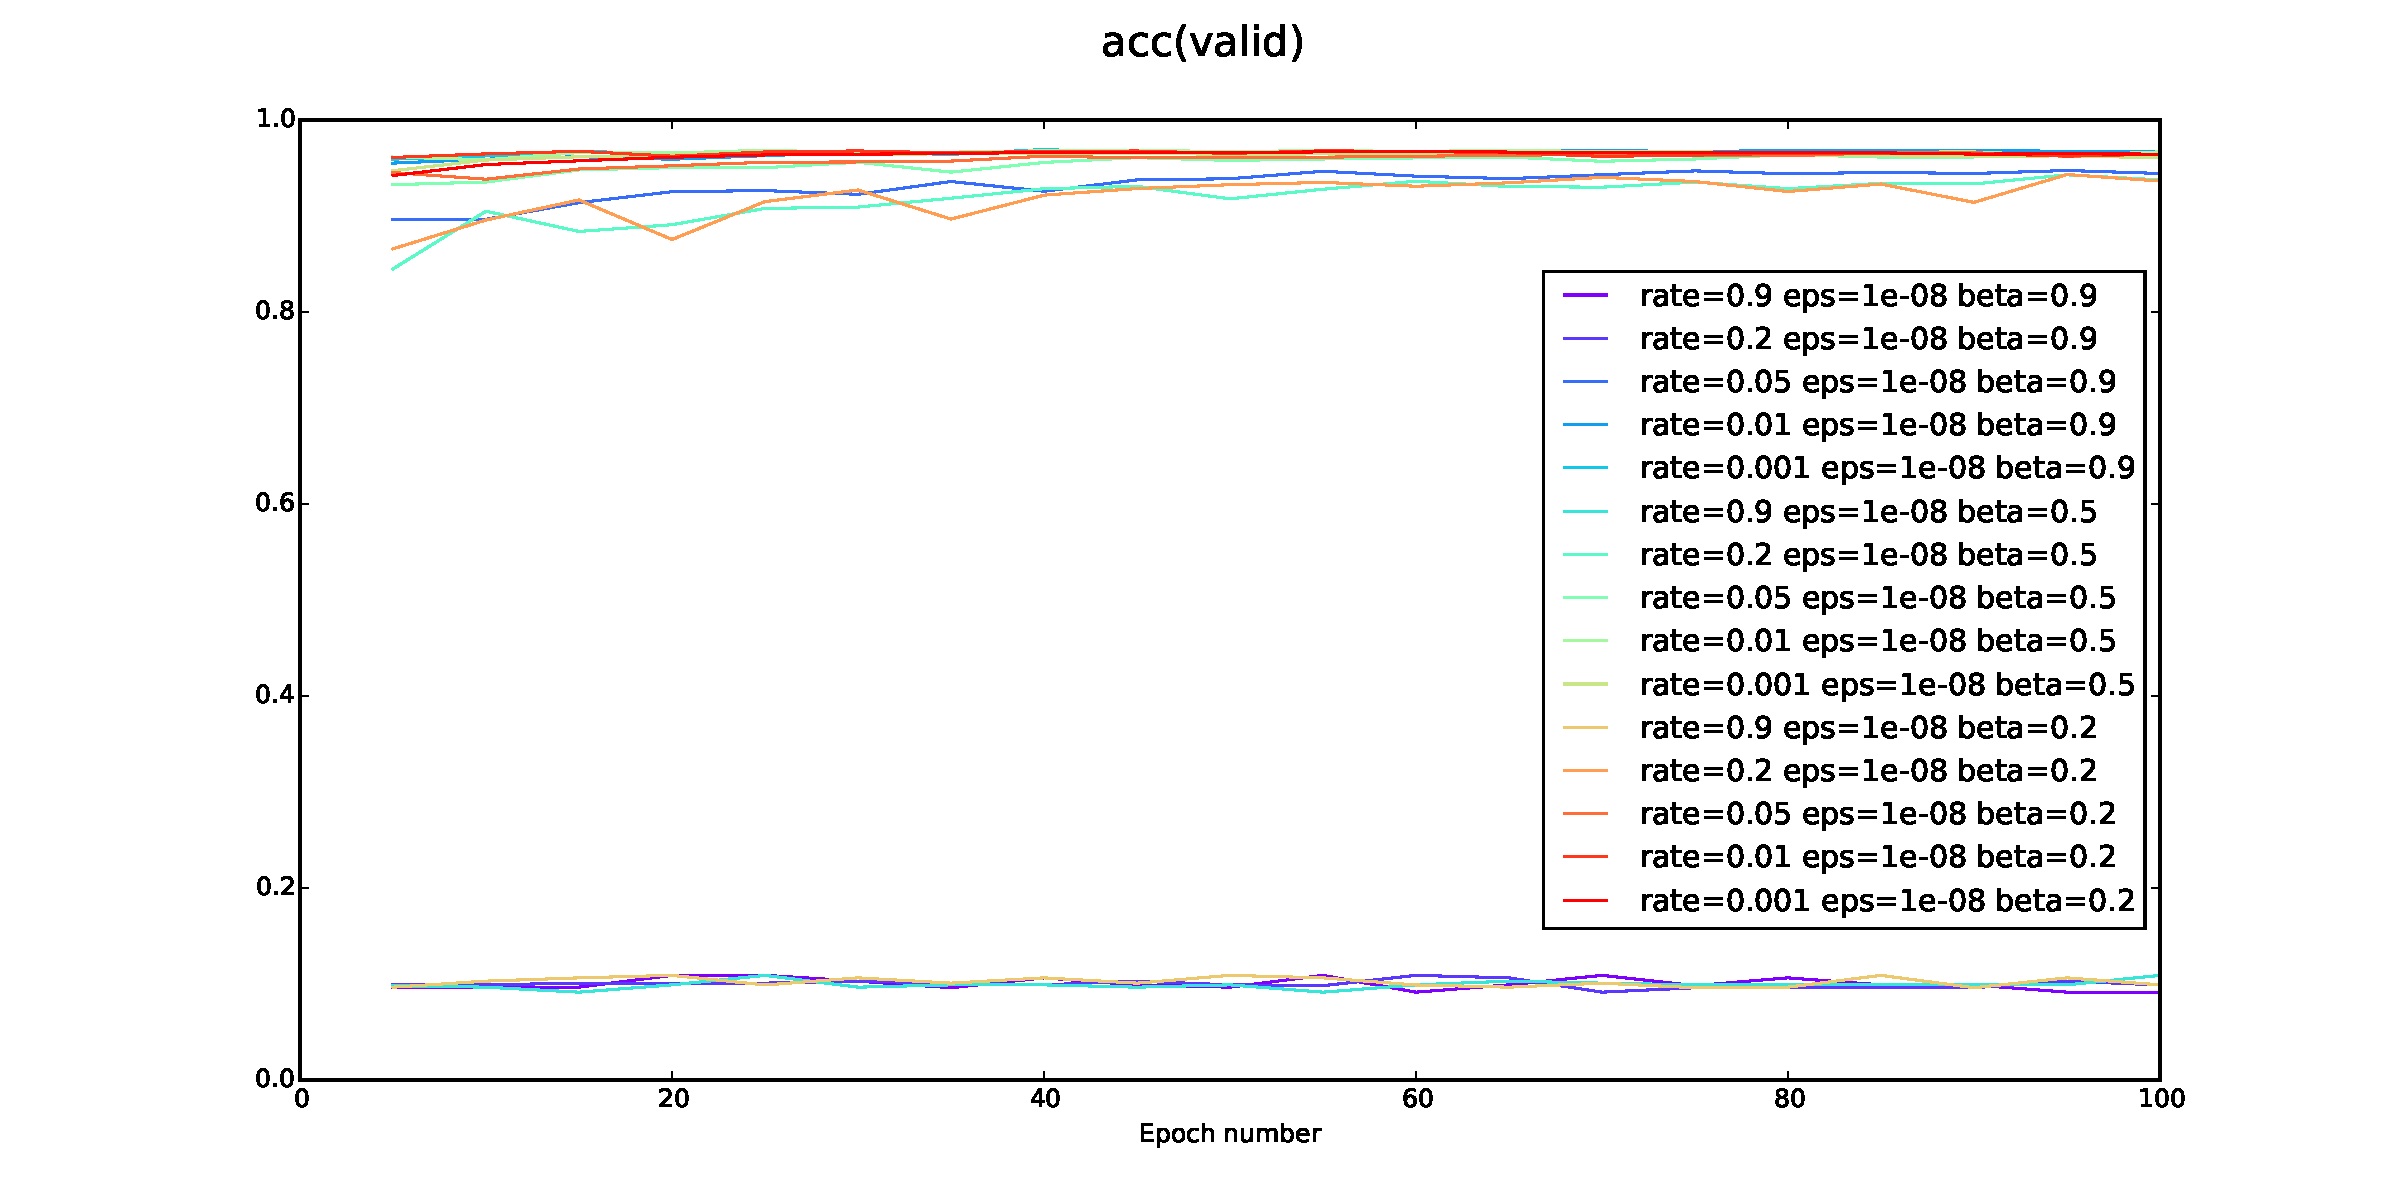
\includegraphics[width=9.1cm]{Task3/figures/Rms_acc(valid).pdf}
\end{subfigure}%
  \caption{RmsProp learning rule hyperparameter results.}
  \label{fig:rms}
\end{figure}

RMSProp is a stochastic gradient descent of RProp. It is also very similar to AdaGrad where it introduces decay rate using the hyperparameter Beta. The effects of Beta are explored in Figure \ref{fig:rms}, showing the best performance with Beta equal to 0.9 which is the commonly accepted value. RMS Prop shows similar performance to AdaGrad and introduces a lot of computational overhead as well for just a small performance boost.
\[ S_i(t) =B*S_i(t-1) + (1-B)*D_i(t)^2\] 
\[ cw_i(t) = -n/(\surd(S_i(t)+e)*D_i(t) \] 

\begin{figure}[h]
\centering
\begin{subfigure}{.5\textwidth}
\centering
\begin{tabular}[h]{| c | c | c |}
\hline
Learning rate & Eps & Accuracy(valid) \\
\hline
1.5 & 1e-08 & 0.099 \\
\hline
1.2 & 1e-08 & 0.099 \\
\hline
0.9 & 1e-08 & 0.099 \\
\hline
0.5 & 1e-08 & 0.929 \\
\hline
0.03 & 1e-08 & 0.9785 \\
\hline
0.2 & 1e-08 & 0.9708 \\
\hline
0.1 & 1e-08 & 0.978 \\
\hline
0.01 & 1e-08 & 0.9718 \\
\hline
1.5 & 1e-06 & 0.099 \\
\hline
1.2 & 1e-06 & 0.099 \\
\hline
0.9 & 1e-06 & 0.099 \\
\hline
0.5 & 1e-06 & 0.099 \\
\hline
0.03 & 1e-06 & 0.9783 \\
\hline
0.2 & 1e-06 & 0.968 \\
\hline
0.1 & 1e-06 & 0.9759 \\
\hline
0.01 & 1e-06 & 0.9719 \\
\hline
\end{tabular}
\end{subfigure}%
\begin{subfigure}{.5\textwidth}

\centering
\begin{tabular}[h]{| c | c | c | c |}
\hline
Learning rate & Eps & Beta & Accuracy(valid) \\
\hline
0.9 & 1e-08 & 0.9 & 0.0915 \\
\hline
0.2 & 1e-08 & 0.9 & 0.099 \\
\hline
0.05 & 1e-08 & 0.9 & 0.9443 \\
\hline
0.01 & 1e-08 & 0.9 & 0.9676 \\
\hline
0.001 & 1e-08 & 0.9 & 0.9618 \\
\hline
0.9 & 1e-08 & 0.5 & 0.109 \\
\hline
0.2 & 1e-08 & 0.5 & 0.9376 \\
\hline
0.05 & 1e-08 & 0.5 & 0.9625 \\
\hline
0.01 & 1e-08 & 0.5 & 0.9668 \\
\hline
0.001 & 1e-08 & 0.5 & 0.9605 \\
\hline
0.9 & 1e-08 & 0.2 & 0.0991 \\
\hline
0.2 & 1e-08 & 0.2 & 0.9364 \\
\hline
0.05 & 1e-08 & 0.2 & 0.9645 \\
\hline
0.01 & 1e-08 & 0.2 & 0.9645 \\
\hline
0.001 & 1e-08 & 0.2 & 0.9645 \\
\hline
\end{tabular}
\end{subfigure}%

  \caption{Comparison of AdaGrad and RMSGrad hyperparameters on accuracy.}
  \label{fig:task3_table}
\end{figure}

\subsection*{Discussion}
Various learning rates, schedules and adaptive learning rates were investigated. Both AdaGrad and RMSProp are the most sophisticated models but they do not provide enough of a value for the computational overhead with the given dataset. Experimenting with different hyperparameters showed that all models can perform very similarly if the right hyperparameters are chosen. This resulted in all models not varying too much from the Baseline as it was performing quite optimally already. The classification misses occurred often at really unclear data points which humans would not really know how to classify themselves. Of all the models explored I would suggest the exponential learning rate decay as it exhibited a convergence speed-up with very little overhead.




\end{document}